\documentclass[sigconf]{acmart}

\usepackage{verbatim}

\usepackage{graphicx}				% Use pdf, png, jpg, or eps§ with pdflatex; use eps in DVI mode
								% TeX will automatically convert eps --> pdf in pdflatex		
\usepackage{amssymb}

\usepackage{algorithm}
\usepackage[noend]{algpseudocode}
\algrenewcommand\textproc{}
%\usepackage[boxed, linesnumbered]{algorithm2e}

\usepackage{array}

\usepackage{subfigure}

\usepackage{epstopdf}

\usepackage{multicol}

\usepackage{balance}

\usepackage{hhline}

%\newtheorem{theorem}{Theorem}%[section]
%\newtheorem{lemma}[theorem]{Lemma}
%\newtheorem{claim}[theorem]{Claim}
%\newtheorem{fact}[theorem]{Fact}
%\newtheorem{definition}[theorem]{Definition}
%\newtheorem{property}[theorem]{Property}

\newcommand{\sq}{\hbox{\rlap{$\sqcap$}$\sqcup$}}
%\newcommand{\qed}{\hspace*{\fill}\sq}

%\newenvironment{proof}{\noindent {\bf Proof.}\ }{\qed\par\vskip 4mm\par}
%\newenvironment{proofof}[1]{\bigskip \noindent {\bf Proof of #1:}\quad }{\qed\par\vskip 4mm\par}

\newcommand{\latpim} {\mathcal{L}_{pim}}
\newcommand{\latcpu} {\mathcal{L}_{cpu}}
\newcommand{\latllc} {\mathcal{L}_{llc}}
\newcommand{\latato} {\mathcal{L}_{atomic}}
\newcommand{\latmes} {\mathcal{L}_{message}}
\newcommand{\Sp}{\mathcal{S}_{p}}


\usepackage{booktabs} % For formal tables


\copyrightyear{2017}
\acmYear{2017}
\setcopyright{acmcopyright}
\acmConference{SPAA '17}{July 24-26, 2017}{Washington DC, USA}
\acmPrice{15.00}
\acmDOI{http://dx.doi.org/10.1145/3087556.3087582}
\acmISBN{978-1-4503-4593-4/17/07}

\clubpenalty = 10000
\widowpenalty = 10000

\begin{document}\sloppy

\title{Concurrent Data Structures for Near-Memory Computing}


\author{Zhiyu Liu}
\affiliation{%
  \institution{Computer Science Department\\
Brown University}
}
\email{zhiyu\_liu@brown.edu}

\author{Irina Calciu}
\affiliation{%
  \institution{VMware Research Group}
}
\email{icalciu@vmware.com}

\author{Maurice Herlihy}
\affiliation{%
  \institution{Computer Science Department\\
Brown University}
}
\email{mph@cs.brown.edu}

\author{Onur Mutlu}
\affiliation{%
  \institution{Computer Science Department\\
ETH Zurich}
}
\email{onur.mutlu@inf.ethz.ch}

% The default list of authors is too long for headers}
%\renewcommand{\shortauthors}{B. Trovato et al.}



\begin{abstract}

The performance gap between memory and CPU has grown exponentially. 
To bridge this gap, hardware architects have proposed 
near-memory computing (also called processing-in-memory, or PIM), 
where a lightweight processor (called a PIM core) is located close to memory. 
Due to its proximity to memory, a memory access from a PIM core is much faster than from a CPU core.
New advances in 3D integration and in die-stacked memory make PIM viable in the 
near future. Prior work has shown significant performance improvements by using PIM for 
embarrassingly parallel and data-intensive applications, as well as for
pointer-chasing traversals in \emph{sequential} data structures. 
However, current server machines have hundreds of cores; algorithms for 
concurrent data structures exploit these cores to achieve high throughput and 
scalability, with significant benefits over sequential data structures. 
No prior work examines the design of concurrent data structures to take the advantage of PIM. 

In this paper, we show two results:
(1) naive PIM data structures cannot outperform state-of-the-art concurrent data structures
such as pointer-chasing data structures and FIFO queue,
(2) novel designs for PIM data structures,
using techniques such as combining, partitioning and pipelining,
can outperform traditional concurrent data structures,
with a significantly simpler design.


\end{abstract}


%
% The code below should be generated by the tool at
% http://dl.acm.org/ccs.cfm
% Please copy and paste the code instead of the example below.
%
%\begin{CCSXML}
%\end{CCSXML}

\keywords{concurrent data structures; parallel programs; processing-in-memory; near-memory computing}

\maketitle

%\section{Introduction}
\section{Near-memory Computing}

The performance gap between memory and CPU has grown exponentially. Memory vendors have focused mostly on improving memory capacity and bandwidth, sometimes even at the cost of increased memory access latencies. To provide higher bandwidth with lower access latencies, hardware architects have proposed near-memory computing (also called \textit{processing-in-memory}, or PIM), where a lightweight processor (called a PIM core) is located close to memory. A memory access from a PIM core is much faster than from a CPU core. 
Near-memory computing is an old idea, that has been intensely studied in the past 
(e.g., \cite{Stone1970, Kogge1994, Gokhale1995, Patterson1997, Oskin1998, KangHYKGLTP99, Hall1999}), 
but so far has not yet materialized. However, new advances in 3D integration and in die stacked memory make near-memory computing viable in the near future. 
For example, one PIM design assumes memory is organized in multiple vaults, each having an in-order PIM core to manage it. These PIM cores
can communicate through message passing, but do not share memory, and cannot access each other's vaults. 

This new technology promises to revolutionize the interaction between computation and data, as memory becomes an active component in managing the data. Therefore, it invites a fundamental rethinking of basic data structures and promotes a tighter dependency between algorithmic design and hardware characteristics. 

Prior work has already shown significant performance improvements by using PIM for embarrassingly parallel 
and data-intensive applications~\cite{Zhang2014:TTP, Ahn2015:2, ZhuASSHPF13, Akin2015:DRM}, 
as well as for pointer-chasing traversals in \emph{sequential} data structures~\cite{hsieh2016accelerating}. 
However, current server machines have hundreds of cores; algorithms for 
concurrent data structures exploit these cores to achieve high throughput and 
scalability, with significant benefits over sequential data structures. 

In this paper, we show that
  naive PIM data structures cannot outperform 
 state-of-the-art \emph{concurrent} data structures. In particular, 
the lower latency access to memory cannot compensate for the loss of 
parallelism. To be competitive with traditional concurrent data structures, 
PIM data structures need new algorithms and new approaches to leverage parallelism.  

But how do we design and optimize data structures for PIM? And how do these algorithms compare to traditional CPU-managed concurrent data structures? To answer these questions, even before the hardware becomes available, we develop a simplified model of the expected performance of PIM. Using this model, we 
investigate two classes of data structures. 

First, in Section~\ref{section:pointer_chasing} we analyze pointer chasing data 
structures, which have a high degree of inherent parallelism and low contention, but incur significant 
overhead due to unpredictable memory accesses. 
We propose using techniques such as combining and partitioning 
the data across vaults to reintroduce parallelism for these data structures.

Second, we explore contended data structures, such as FIFO queues (Section~\ref{section:contended}), 
which can leverage CPU caches to exploit their inherent high locality. 
Therefore, FIFO queues might not seem to be able to leverage PIM's faster memory accesses. 
Nevertheless, these data structures exhibit a high degree of contention, which makes it difficult even for 
the most advanced algorithms to obtain good performance for many threads accessing the data concurrently. 
We use pipelining of requests, which can be done very efficiently in PIM, to design a new FIFO queue 
suitable for PIM that can outperform state-of-the-art concurrent FIFO queues~\cite{Morrison13, Hendler10}.

The contributions of this paper are summarized below.
\begin{itemize}
\item We propose a very simple model to analyze performance of PIM data structures and
concurrent data structures based on the latency of a memory access and an estimated number of 
accesses served from the cache, as well as the number of atomic operations used. 
\item Using this model, we show that the lower latencies are not sufficient for PIM data structures
to outperform efficient concurrent algorithms. 
 \item We propose new designs for PIM 
data structures using 
techniques such as combining, partitioning and pipelining, that can outperform traditional 
concurrent data structures, with a significantly simpler design. 
\end{itemize}


The paper is organized as follows. In Section~\ref{section:hardware_model} we briefly describe 
our assumptions about the hardware architecture. 
In Section~\ref{section:performance_model} we introduce a simplified performance model 
that we use throughout this paper to predict performance of our algorithms using the hardware 
architecture described in Section~\ref{section:hardware_model}. 
Next, in Sections~\ref{section:pointer_chasing} and \ref{section:contended}, 
we describe and analyze our PIM algorithms and use our model to compare them to prior work. 
We also use current architectures to simulate the behavior of our algorithms and 
evaluate compared to state-of-the-art concurrent algorithms. 
Finally, we present related work in Section~\ref{section:related_work} 
and conclude in Section~\ref{section:conclusion}. 


\section{Processing in Memory}
\label{section:model}

\subsection{Hardware model}
\label{section:hardware_model}

\begin{figure}[ht!]
%$\hrulefill$
%\\
%\\
\centering
\includegraphics[width=.9\linewidth]{model.eps}
%$\hrulefill$
\caption{The PIM model}
\label{figure:model}
\end{figure}

In the PIM hardware model, multiple CPUs are connected to the main
memory, via a shared crossbar network, as illustrated in Figure \ref{figure:model}.
The main memory consists of two parts---one is a normal DRAM accessible by CPUs 
and the other, called the \textit{PIM memory}, is divided into multiple partitions, 
called \textit{PIM vaults} or simply vaults.  
According to the Hybrid Memory Cube specification 1.0 \cite{website:HMC}, each HMC consists of 16 or 
32 vaults and has total size 2GB or 4 GB (so each vault has size roughly 100MB). 
We assume the same specifications in our PIM model, although the size of a PIM memory and 
the number of its vaults can be greater in theory. 
Each CPU also has access to a hierarchy of cache, coherent to the normal DRAM, 
and the last-level cache is shared among CPUs. 

Each vault has a \textit{PIM core} directly attached to it.
we say a vault is \textit{local} to the PIM core attached to it, and vice versa.
A PIM core is a lightweight CPU that may be slower than a full-fledged CPU
with respect to computation speed.\footnote{
A PIM core can be thought of as an in-order CPU with only small private L1 cache and 
without some optimizations that full-fledged CPUs usually have.}
A vault can be accessed only by its local PIM core.\footnote{
We may alternatively assume that a PIM core has direct access to remote vaults, at a larger cost. 
We may also assume that vaults are accessible by CPUs as well, 
but at the cost of dealing with cache coherence between CPUs and PIM cores. 
Some cache coherence mechanisms for PIM memory have be proposed 
and claimed to be not costly (e.g., \cite{boroumand2016}). 
However, we prefer to keep the hardware model simple and we will show that we are still able to 
design efficient concurrent data structure algorithms with this simple, less powerful PIM memory.}
Although a PIM core is relatively slow computationally, it has fast access to its local vault.

A PIM core communicates with other PIM cores and CPUs via messages.
Each PIM core, as well as each CPU, has buffers for storing incoming messages.
A message is guaranteed to eventually arrive at the buffer of its receiver.
Messages from the same sender to the same receiver are delivered in FIFO order: 
the message sent first arrives at the receiver first. 
However, messages from different senders or to different receivers can arrive in an arbitrary order. 

To keep the PIM memory simple, we assume that a PIM core can only make read and write operations 
to its local vault, while a CPU also supports more powerful atomic operations, such as CAS and F\&A.
Virtual memory is cheap to be achieved in this model, 
by having each PIM core maintain its own page table for its local vault.
\section{Performance Model}
%\subsection{Performance model}
\label{section:performance_model}
Based on the latency numbers in prior work on PIM memory, 
in particular on the Hybrid Memory Cube \cite{website:HMC, Azarkhish16}, 
and on the evalutation of operations in multiprocessor architectures \cite{David13},
we propose the following simple performance model to compare 
our PIM-managed algorithms with existing concurrent data structure algorithms.
For read and write operations, we assume 
$$\latcpu = 3\latpim = 3\latllc,$$
where $\latcpu$ is the latency of a memory access by a CPU,
$\latpim$ is the latency of a local memory access by a PIM core, and
$\latllc$ is the latency of a last-level cache access by a CPU.
We ignore the costs of cache accesses of other levels in our performance model,
as they are negligible in the concurrent data structure algorithms we will consider.
We assume that the latency of a CPU making an atomic operation, such as a CAS or a F\&A,
to a cache line is 
$$\latato = \latcpu,$$ 
even if the cache line is currently in cache.
This is because an atomic operation hitting the cache is usually 
as costly as a memory access by a CPU, acorrding to \cite{David13}.
When there are $k$ atomic operations competing for a cache line concurrently,
we assume that they are executed sequentially, that is,
they complete in times $\latato, 2\latato,..., k\cdot\latato$, respectively.

We assume that the size of a message sent by a PIM core or a CPU is at most 
the size of a cache line.
Given that a message transferred between a CPU and a PIM core goes through
the crossbar network, we assume that the latency for a message to arrive at its receiver is 
$$\latmes = \latcpu.$$
We make a conservative assumption that the latency of a message transferred 
between two PIM cores is also $\latmes$.
Note that the message latency we consider here is the transfer time of a message
through a message passing channel, that is, the period between the moment
when a PIM or a CPU sends off the message and the moment when
the message arrives at the buffer of its receiver.
We ignore the time spent in other parts of a message passing procedure,
such as preprocessing and constructing the message,
as it is negligible compared to the time spent in message transfer.



%\section{Pointer-Chasing Data Structures}
\section{Low Contention Data \\ Structures}
\label{section:pointer_chasing}

In this section we consider data structures with low contention; pointer chasing data structures, 
such as linked-lists and skip-lists, fall in this category.  
These are data structures whose operations  
need to de-reference a non-constant sequence of pointers before completing. We assume they support operations 
such as add($x$), delete($x$) and contains($x$), which follow ``next node" pointers until 
reaching the position of node $x$.
When these data structures are too large to fit in CPU caches 
and access uniformly random keys,
they incur expensive memory accesses, which cannot
be easily predicted, making the pointer chasing the dominating overhead of these data structures.
Naturally, these data structures have been early examples of the benefit of near-memory 
computing~\cite{}, as the entire pointer chase could be performed by the PIM core, and only the final result returned to 
the application. 

However, under the same conditions, these data structures have inherently low contetion. Lock-free algorithms~\cite{}
have shown that these data structures can scale to hundreds of cores under low contention. Unfortunately, each vault in 
PIM memory has a single core; as a consequence, prior work 
has only compared PIM data structures with sequential data structures, 
not with carefully crafted concurrent data structures.

We analyze linked-lists and skip-lists, and show that the naive PIM data structure in each case cannot 
outperform the equivalent CPU managed concurrent data structure even for a small number of cores. Next, 
we show how to use state-of-the art techniques from concurrent computing literature to 
optimize algorithms for near-memory computing to outperform well-known concurrent data 
structures. 

%\subsection{PIM-managed linked-list}
\subsection{Linked-lists}
\label{section:linked_list}
We now describe a naive PIM linked-list.
The linked-list is stored in a vault, maintained by the local PIM core.
Whenever a CPU\footnote{We use the term CPU to refer to CPU cores, as oposed to PIM cores.} 
wants to perform an operation on the linked-list,
it sends a request to the PIM core.
The PIM core will retrieve the message, execute the operation, and send the result back to the CPU.
The PIM linked-list is sequential, as it can only be accessed by one PIM core. 

Doing pointer chasing on sequential data structures by PIM cores is not a new idea
(e.g., \cite{hsieh2016accelerating, Ahn2015:2}).
It is obvious that for a sequential data structure like a sequential linked-list,
replacing the CPU with a PIM core to access the data structure will largely improve
its performance due to the PIM core's much faster memory access.
However, we are not aware of any prior comparison between the performance of
PIM-managed data structures and concurrent data structures
in which CPUs can make operations in parallel.
In fact, our analytical and experimental results will show that
the performance of the naive PIM-managed linked-list is much worse than
that of the concurrent linked-list with fine-grained locks \cite{Heller05}.

To improve the performance of the PIM-managed linked-list,
we apply the following \textit{combining optimization} to it:
the PIM core retrieves all pending requests from its buffer and
executes all of them during only one traversal over the linked-list.
It is not hard to see that the role of the PIM core in our PIM-managed linked-list
is very similar to that of the combiner in a concurrent linked-list implemented
using \textit{flat combining} \cite{Hendler10}, where, roughly speaking,
threads compete for a ``combiner lock" to become the combiner, and
the combiner will take over all operation requests from other threads and execute them.
Therefore, we think the performance of the flat-combining linked-list is a good indicator to
the performance of our PIM-managed linked-list.

Based on our performance model, we can calculate the approximate expected
throughputs of the linked-list algorithms mentioned above, 
when there are $p$ CPUs making operation requests concurrently.
We assume that a linked-list consists of nodes with integer keys in the range of $[1, N]$.
Initially a linked-list has $n$ nodes with keys generated independently
and uniformly at random from $[1, N]$.
The keys of the operation requests are generated the same way.
To simplify the analysis, we assume that CPUs only make $contains()$ requests
(or the number of $add()$ requests is the same as the number of $delete()$
so that the size of each linked-list nearly doesn't change).
We also assume that a CPU makes a new operation request immediately after
its previous one completes.
Assuming that $n \gg p$ and $N \gg p$, the approximate expected throughputs (per second) 
of the concurrent linked-lists are presented in Table \ref{tab:linkedlist}, 
where $\Sp = \sum\limits_{i=1}^{n} ({i \over n+1})^{p}$.\footnote{
We define the rank of an operation request to a linked-list as the number of pointers
it has to traverse until it finds the right position for it in the linked-list.
$\Sp$ is the expected rank of the operation request with the biggest key
among $p$ random requests a PIM core or a combiner has to combine,
which is essentially the expected number of pointers a PIM core or a combiner
has to go through during one pointer chasing procedure.}

\begin{table}[ht!]
\begin{center}
    \begin{tabular}{| >{\small}l | l |}
    \hline
    Algorithm & Throughput\\ \hline
    Linked-list with fine-grained locks & ${2p \over (n+1)\latcpu}$ \\ \hline
    Flat-combining linked-list without combining & ${2 \over (n+1)\latcpu}$ \\ \hline
    PIM-managed linked-list without combining & ${2 \over (n+1)\latpim}$ \\ \hline
    Flat-combining linked-list with combining & ${p \over (n-\Sp)\latcpu}$ \\ \hline
    PIM-managed linked-list with combining & ${p \over (n-\Sp)\latpim}$ \\ \hline
    \end{tabular}
\end{center}
\caption{Throughputs of linked-list algorithms.}
\label{tab:linkedlist}
\end{table}


It is easy to see that the PIM-managed linked-list with combining outperforms 
the linked-list with fine-grained locks, which is the best one among other algorithms, 
as long as ${\latcpu \over \latpim} > {2(n - \Sp)\over n + 1}$.
Given that $0 < \Sp \le {n \over 2}$ and $\latcpu = 3\latpim$,
the throughput of the PIM-managed linked-list with combining should be at least 
1.5 times the throughput of the linked-list with fine-grained locks.
Without combining, however, the PIM-managed linked-list cannot
beat the linked-list with fine-grained locks when $p > 6$.

We implemented the linked-list with fine-grained locks and the flat-combining link-list 
with and without the combining optimization.
We tested them on a Dell server with 512 GB RAM and 
56 cores on four Intel Xeon E7-4850v3 processors at 2.2 GHz.
To get rid of NUMA access effects, we ran experiments with only one processor, 
which is a NUMA node with 14 cores, a 35 MB shared L3 cache, 
and a private L2/L1 cache of size 256 KB/64 KB per core. 
Each core has 2 hyperthreads, for a total of 28 hyperthreads. 
Cache lines have 64 bytes.

The throughputs of the algorithms are presented in Figure \ref{figure:linkedlist_data}.
The results confirmed the validity of our analysis in Table \ref{tab:linkedlist}.
The throughput of the flat-combining algorithm without combining optimization
is much worse than the algorithm with fine-grained locks.
Since we believe the performance of the flat-combining linked-list is a good 
indicator of that of the PIM-managed linked-list, we triple the throughput of the
flat-combining algorithm without combining optimization to get the estimated
throughput of the PIM-managed algorithm. 
As we can see, it is still far below the throughput of the one with fined-grained locks.
However, with the combining optimization, the performance of the flat-combining
algorithm improves significantly and the estimated throughput of our PIM-managed
linked-list with combining optimization now beats all others'.

\begin{comment}
\begin{figure}[ht!]
    \centering
    \begin{minipage}{0.45\linewidth}
        \centering
        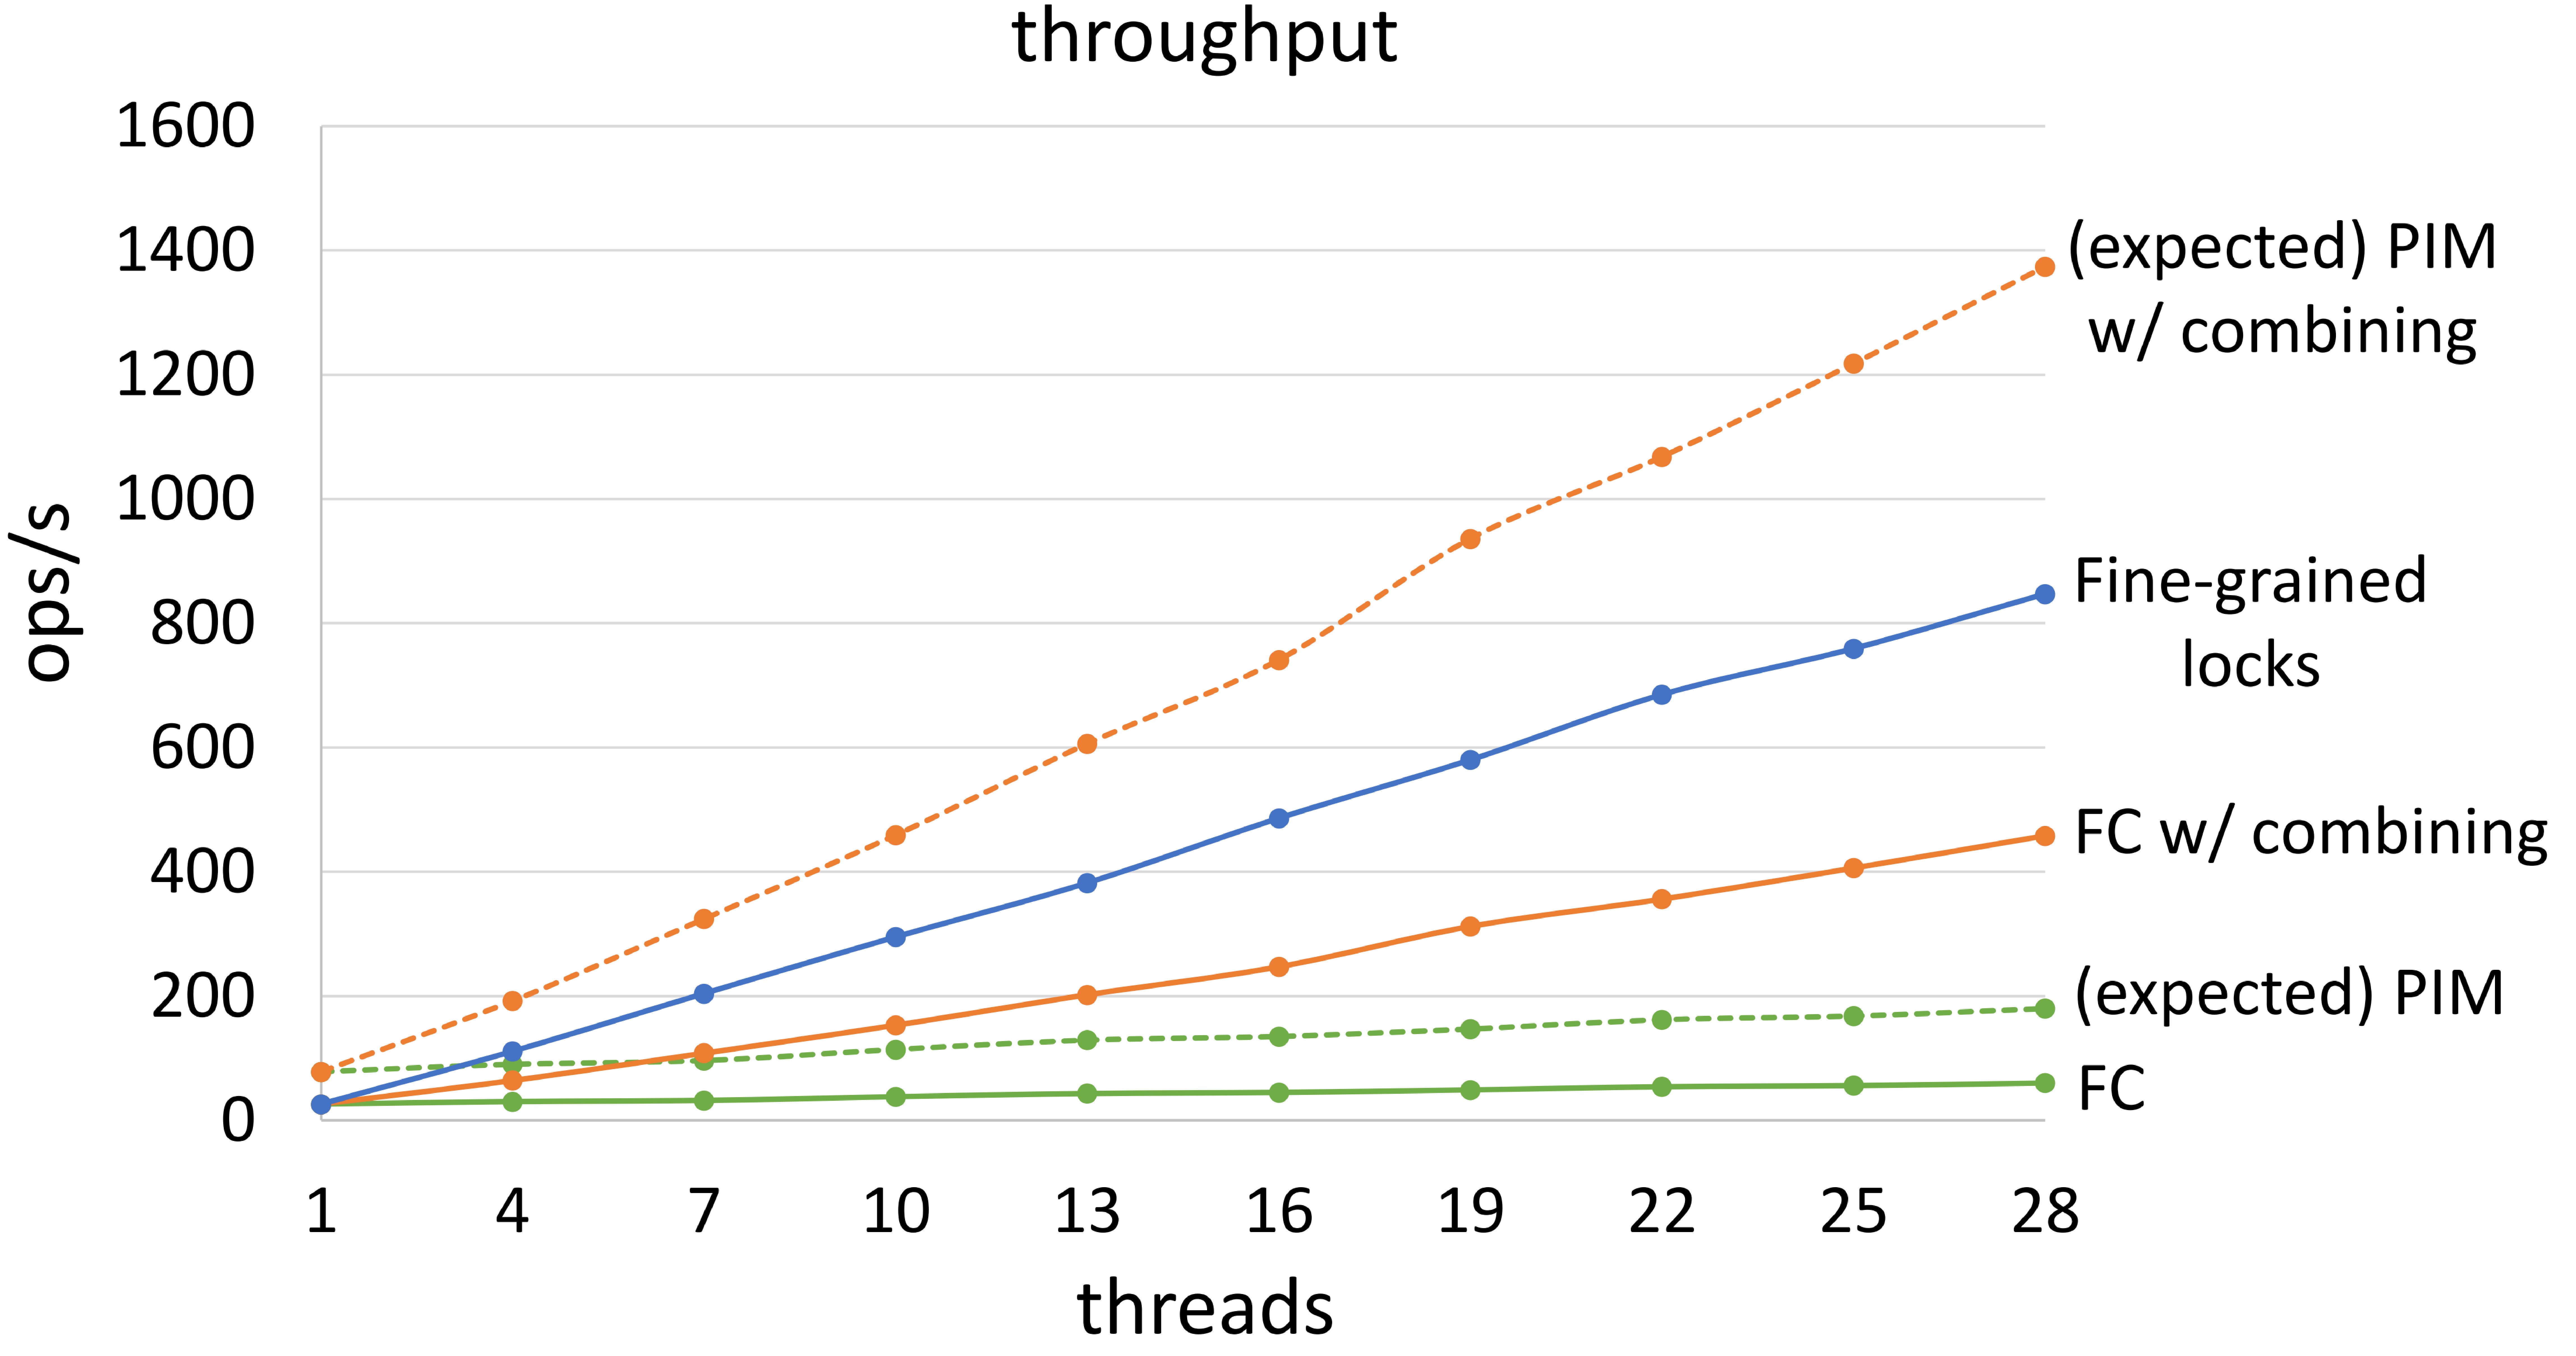
\includegraphics[width=.9\linewidth]{linkedlist_data.eps} % first figure itself
        \caption{Experimental results of linked-lists}
        \label{figure:linkedlist_data}
    \end{minipage}\hfill
    \begin{minipage}{0.45\linewidth}
        \centering
        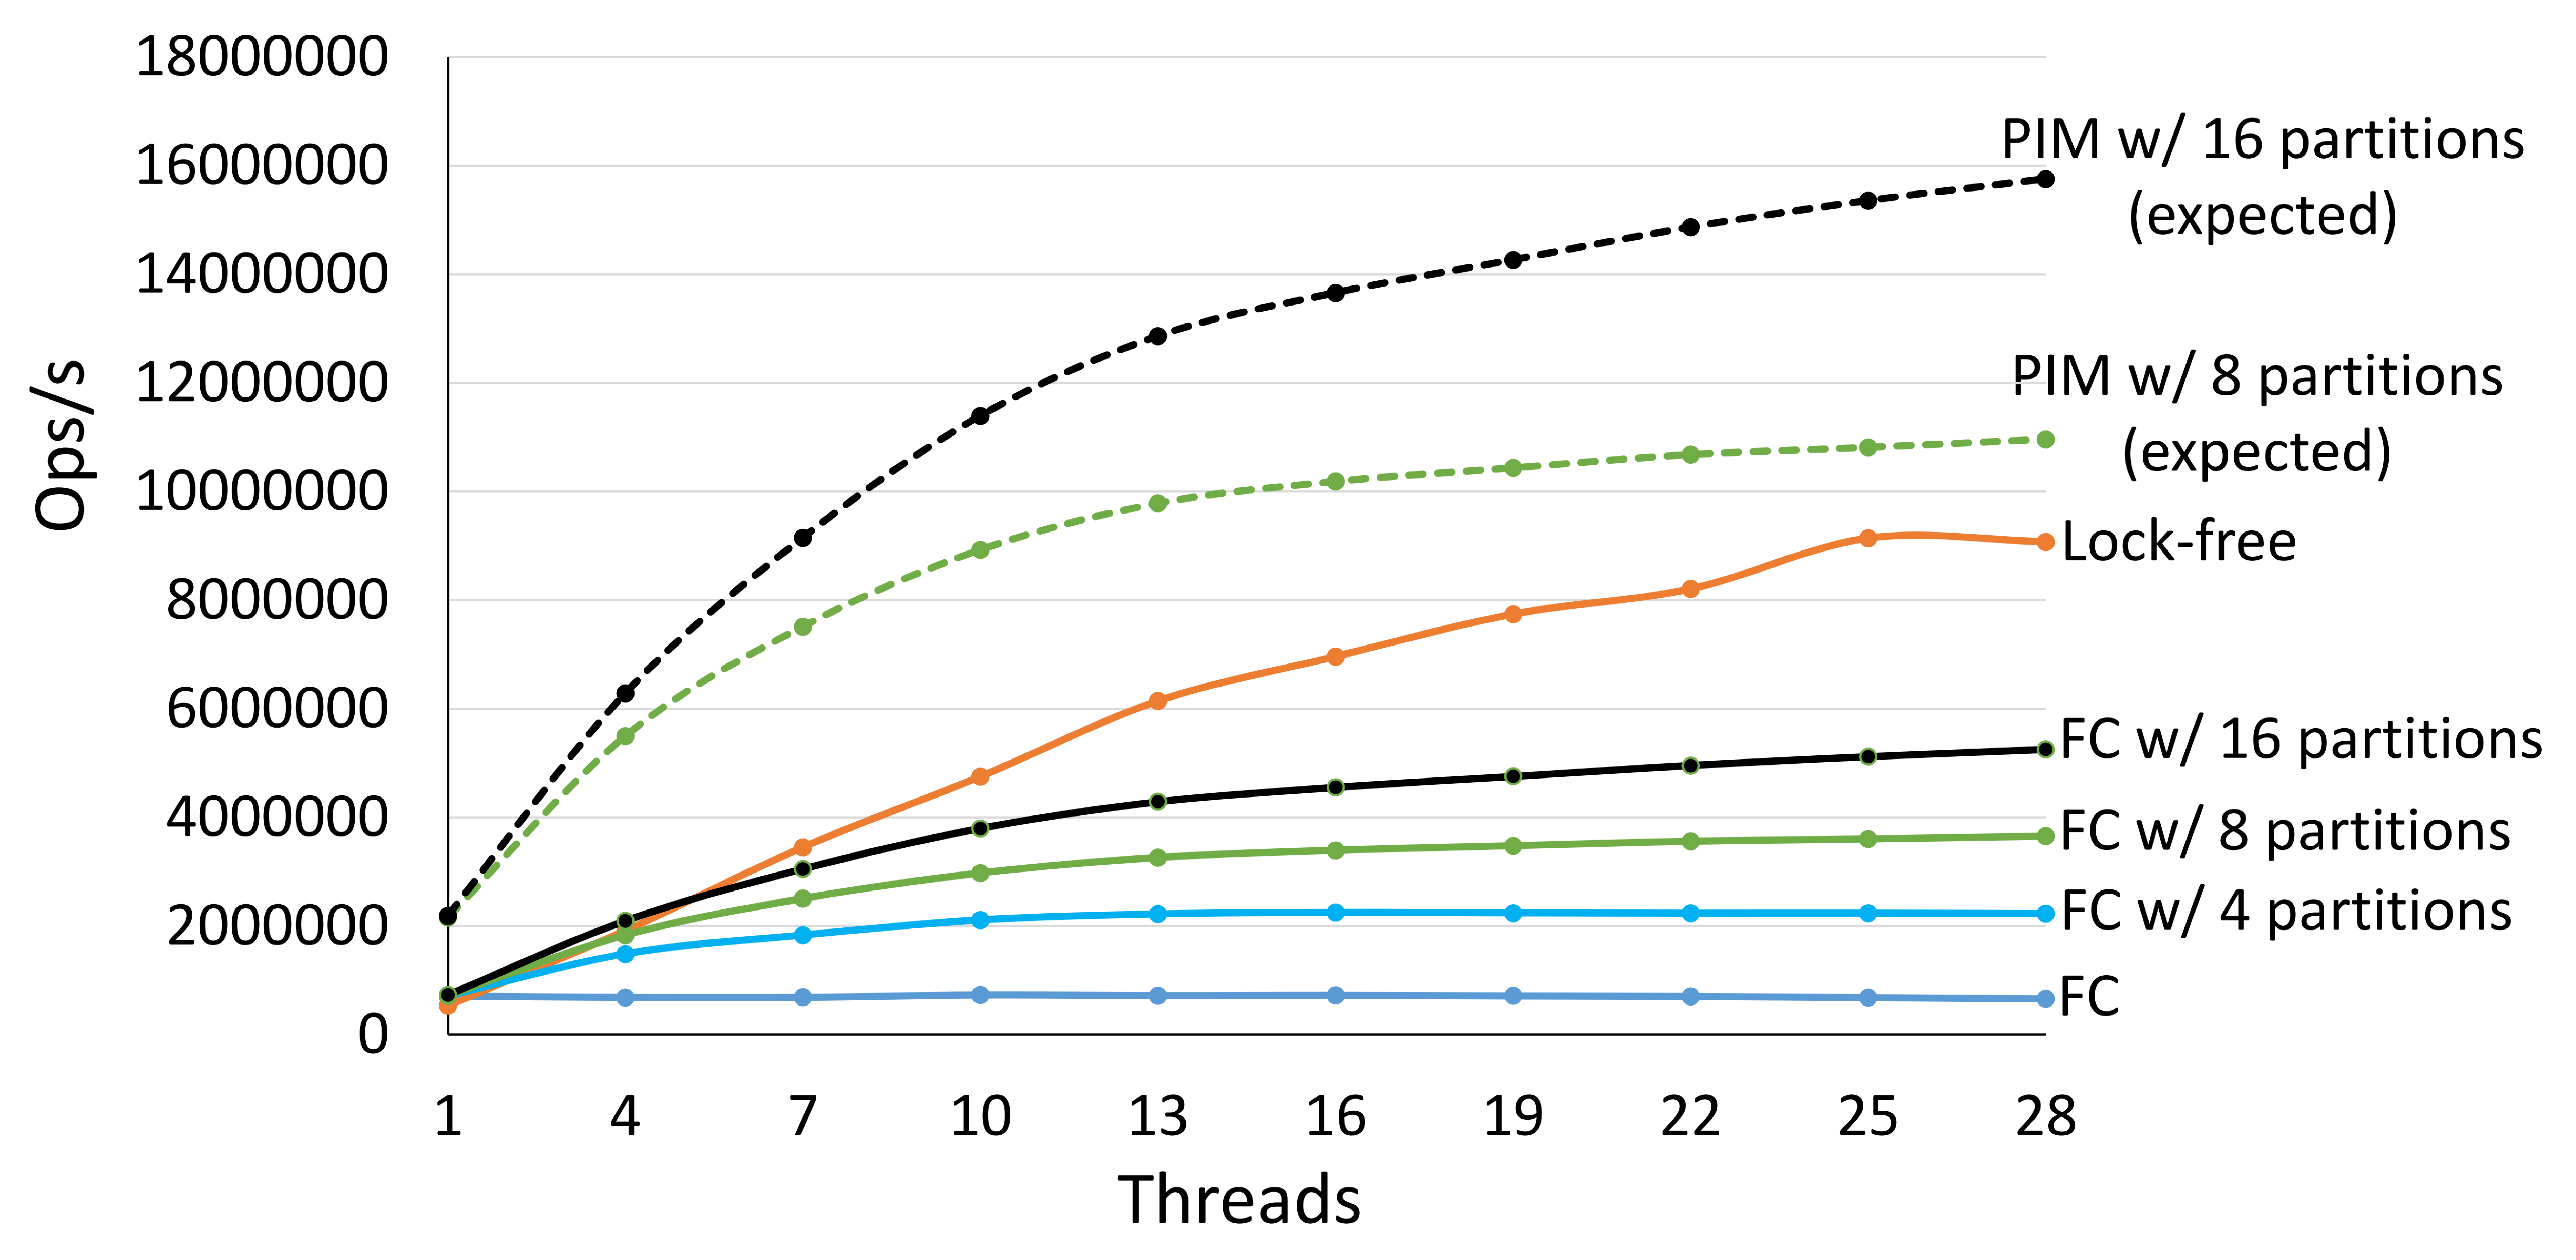
\includegraphics[width=.98\linewidth]{skiplist_data.eps} % second figure itself
        \caption{Experimental results of skip-lists}
        \label{figure:skiplist_data}
    \end{minipage}
\end{figure}
\end{comment}

\begin{figure}[ht!]
    \centering
    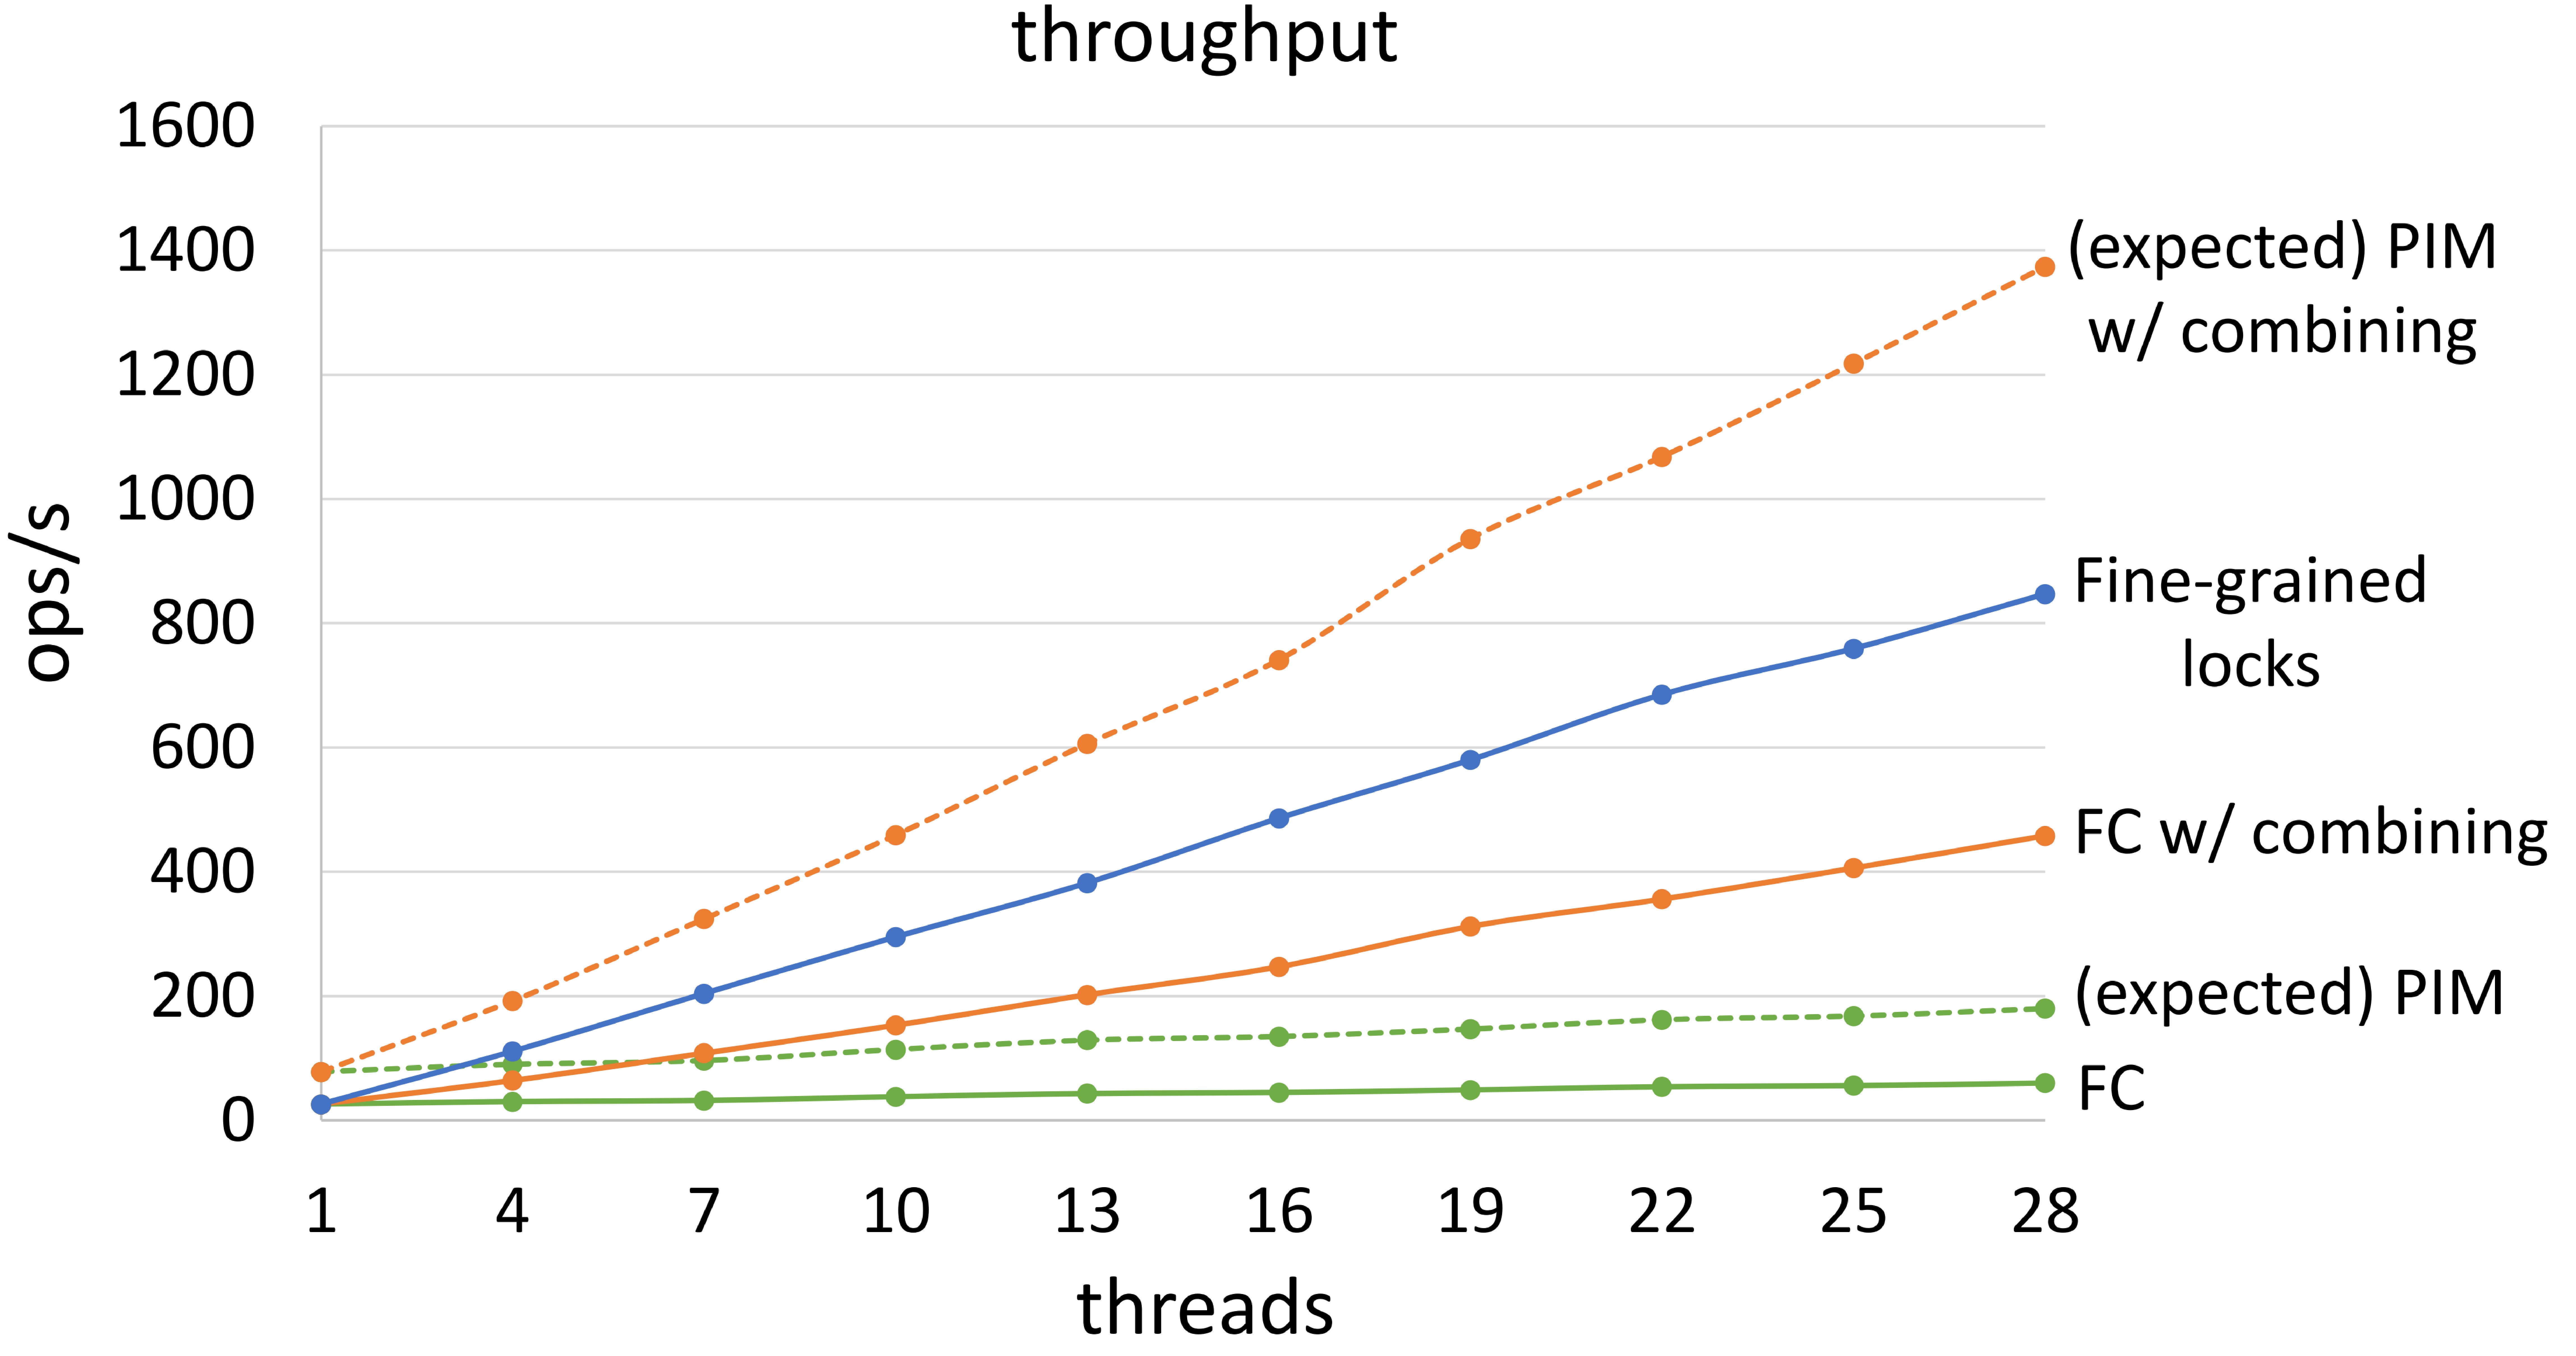
\includegraphics[width=1.0\linewidth]{linkedlist_data.eps} % first figure itself
    \caption{Experimental results of linked-lists. We evaluated the linked-list with Fine-grained locks 
        and the flat-combining linked-list (FC) with and without the combining optimization.}
   \label{figure:linkedlist_data}
\end{figure}


\subsection{Skip-lists}
\label{section:skip_list}

%\subsubsection{Base algorithm}

Like the naive PIM-managed linked-list,
the naive PIM-managed skip-list keeps the skip-list in a single vault and
CPUs send operation requests to the local PIM core that executes those operations.
As we will see, this algorithm is less efficient than some existing algorithms.

Unfortunately, the combining optimization cannot be applied to skip-lists effectively.
The reason is that for any two nodes not close enough to each other in the skip-list,
the paths we traverse through to reach them don't largely overlap.

On the other hand, PIM memory usually consists of many vaults and PIM cores.
For instance, the first generation of Hybrid Memory Cube \cite{website:HMC} has up to 32 vaults.
Hence, a PIM-managed skip-list may achieve much better performance if
we can exploit the parallelism of multiple vaults.
Here we present our PIM-managed skip-list with a \textit{partitioning optimization}:
A skip-list is divided into partitions of disjoint ranges of keys,
stored in different vaults, so that a CPU sends its operation request to
the PIM core of the vault to which the key of the operation belongs.

Figure \ref{figure:skiplist_structure} illustrates the structure of a PIM-managed skip-list.
Each partition of a skip-list starts with a \textit{sentinel node}
which is a node of the max height. 
For simplicity, assume the max height $H_{max}$ is predefined.
A partition covers a key range between the key of its sentinel node and
the key of the sentinel node of the next partition.
CPUs also store a copy of each sentinel node in the normal DRAM and 
the copy has an extra variable indicating the vault containing the sentinel node.
Since the number of nodes of the max height is very small with high probability, 
those copies of those sentinel nodes can almost certainly stay in cache
if CPUs access them frequently.

When a CPU applies an operation for a key to the skip-list,
it first compares the key with those of the sentinels, discovers which vault
the key belongs to, and then sends its operation request to that vault's PIM core.
Once the PIM core retrieves the request, it executes the operation in the local vault 
and finally sends the result back to the CPU.


\begin{figure}[ht!]
%$\hrulefill$
%\\
%\\
\centering
\includegraphics[width=1.0\linewidth]{skiplist_structure.eps}
%$\hrulefill$
\caption{A PIM-managed FIFO queue with three partitions}
\label{figure:skiplist_structure}
\end{figure}

Now let us discuss how we implement the PIM-managed skip-list
when the key of each operation is an integer generated uniformly at random
from range $[0, n]$ and the PIM memory has $k$ vaults available.
Initially we can create $k$ partitions starting with fake sentinel nodes
with keys $0$, $1/k$, $2/k$,..., $(n-1)/k$, respectively, 
and allocate each partition in a different vault. 
The sentinel nodes will never be deleted.
If a new node to be added has the same key as a sentinel node,
we insert it immediately after the sentinel node.

We compare the performance of our PIM-managed skip-list with partitions 
to the performance of a flat-combining skip-list \cite{Hendler10}
and a lock-free skip-list \cite{Herlihy08}, 
where $p$ CPUs keeps making operation requests.
We also apply the partitioning optimization to the flat-combining skip-list, 
so that $k$ combiners are in charge of $k$ partitions of the skip-list. 
To simplify the comparison, we assume that all skip-lists have the same
initial structure (expect that skip-lists with partitions have extra sentinel nodes)
and all the operations are contains() operations
(or the number of $add()$ requests is the same as the number of $delete()$ 
so that the size of each skip-list nearly doesn't change).
Their approximate expected throughputs are presented in Table \ref{tab:skiplist}, 
where $\beta$ is the average number of nodes an operation has to go through
in order to find the location of its key in a skip-list
($\beta = \Theta(\log N)$, where $N$ is the size of the skip-list).
Note that we have ignored some overheads in the flat-combining
algorithms, such as maintaining combiner locks and publication lists
(we will discuss publication lists in more detail in Section \ref{section:contended}).
We also have overestimated the performance of the lock-free skip-list by not counting the
CAS operations used in add() and delete() requests, as well as the cost of retries
caused by conflicts of updates.
Even so, our PIM-managed linked-list with partitioning optimization is
still expected to outperform the second best algorithm, the lock-free skip-list 
when $k > {(\beta\latpim + \latmes)p \over \beta\latcpu}$.
Given that $\latmes = \latcpu = 3\latpim$, $k > p/3$ should suffice.

\begin{table}[ht!]
\begin{center}
	\begin{tabular}{| >{\small}l | l |}
    %\begin{tabular}{| m{0.68\linewidth}  | l |}
    \hline
    Algorithm & Throughput\\ \hline
    Look-free skip-list & ${p \over \beta\latcpu}$ \\ \hline
    Flat-combining skip-list & ${1 \over \beta\latcpu}$ \\ \hline
    PIM-managed skip-list & ${1 \over (\beta\latpim + \latmes)}$ \\ \hline
    Flat-combining skip-list with $k$ partitions & ${k \over \beta\latcpu}$ \\ \hline
    PIM-managed skip-list with $k$ partitions & ${k \over (\beta\latpim + \latmes)}$ \\ \hline
    \end{tabular}
\end{center}
\caption{Throughputs of skip-list algorithms.}
\label{tab:skiplist}
\end{table}

Our experiments have revealed similar results, 
as presented in Figure \ref{figure:skiplist_data}.
We have implemented and run the flat-combining skip-list with different numbers of
partitions and compared them with the lock-free skip-list.
As the number of partitions increases, the performance of the flat-combining skip-list
gets better, implying the effectiveness of the partitioning optimization.
Again we believe the performance of the flat-combining skip-list is a good indicator
to the performance of our PIM-managed skip-list.
Therefore, according to the analytical results in Table \ref{tab:skiplist}, we can triple the throughput 
of a flat-combining skip-list to get the expected performance of a PIM-managed skip-list.
As Figure \ref{figure:skiplist_data} illustrates, when the PIM-managed skip-list has $8$ or $16$ 
partitions, it is expected to outperform the lock-free skip-list with up to 28 hardware threads.

\begin{figure}[ht!]
    \centering
    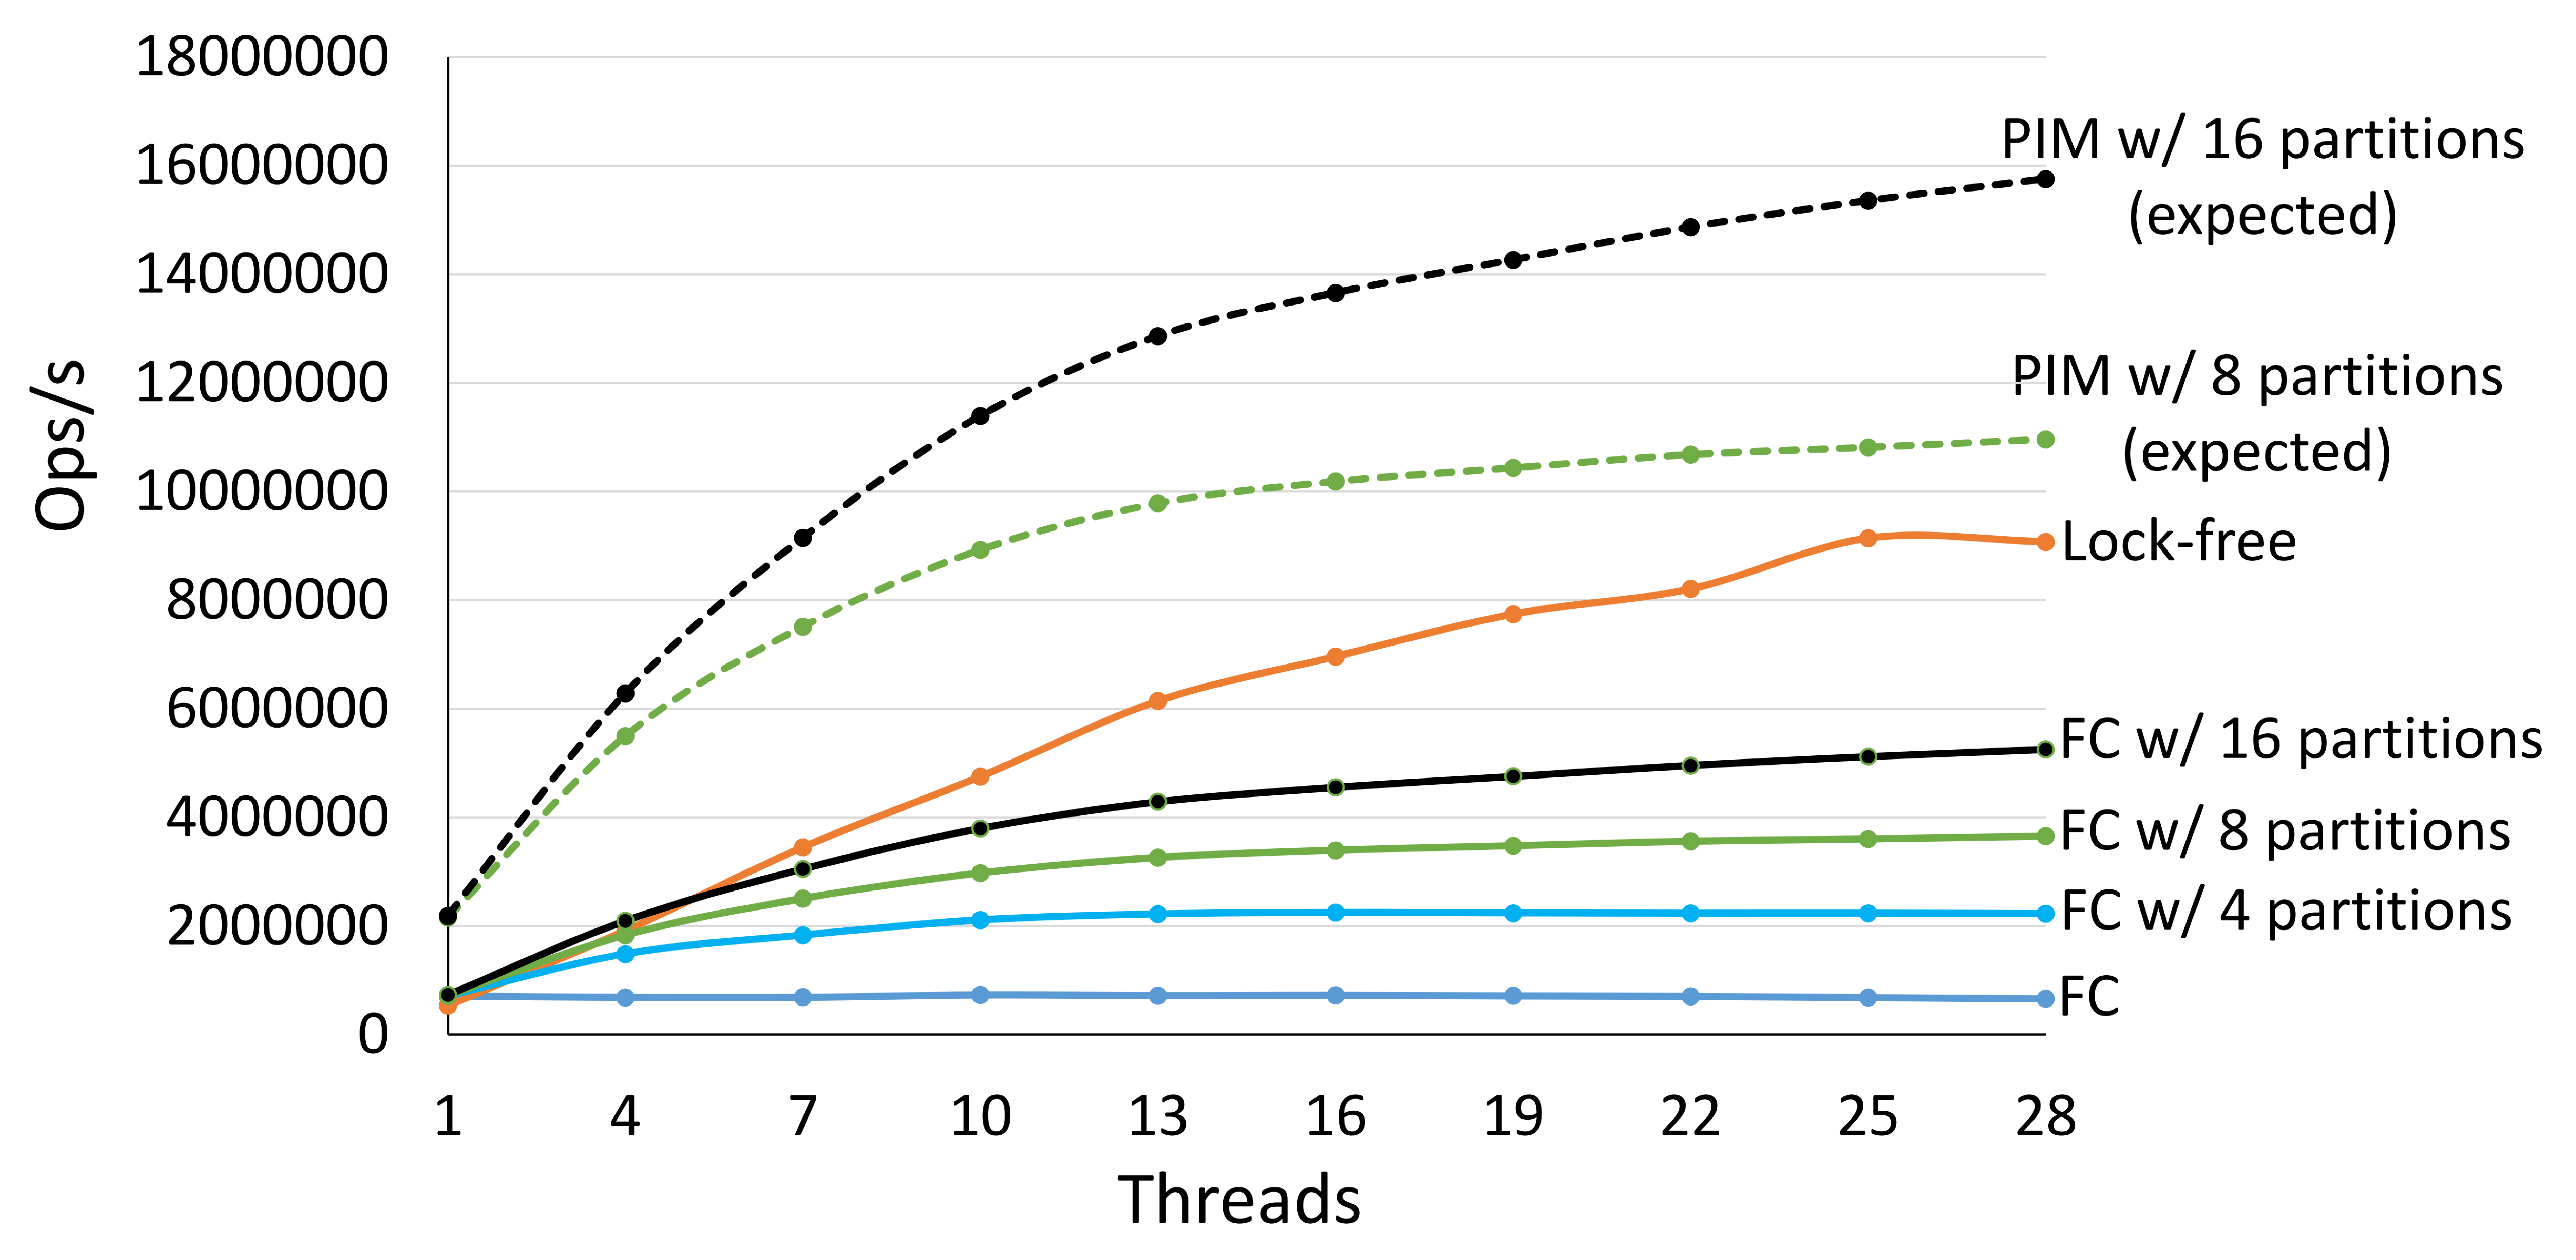
\includegraphics[width=1.0\linewidth]{skiplist_data.eps} % second figure itself
    \caption{Experimental results of skip-lists. We evaluated the lock-free skip-list and 
    the flat-combining skip-list (FC) with different numbers (1, 4, 8, 16) of partitions.}
    \label{figure:skiplist_data}
\end{figure}


%\subsubsection{Rebalancing skip-list}
\subsubsection{Skip-list Rebalancing}
The PIM-managed skip-list performs well with a uniform distribution of requests.
However, if the distribution of requests is not uniform, a static partitioning scheme 
will result in unbalanced partitions, with some PIM cores being idle, while others having to 
serve a majority of requests. To address this problem, we introduce a non-blocking protocol for 
migrating consecutive nodes from one vault to another. 

The protocol works as follows. 
A PIM core $p$ that manages a vault $v'$ can send a message to another PIM core $q$, managing vault 
$v$, to request that some nodes are moved from $v'$ to $v$. 
First, $p$ sends a message notifying $q$ of the start of the migration. 
Then $p$ sends messages of adding those nodes to $q$ one by one in an ascending order 
according to the keys of the nodes. 
After all the nodes have been migrated, $p$ sends notification messages to CPUs so that 
they can update their copies of sentinel nodes accordingly.
After $p$ receives acknowledgement messages from all CPUs, it notifies $q$ of the end of migration.
To keep the node migration protocol simple, we don't allow $q$ to move those nodes 
to another vault again until $p$ finishes its node migration. 

During the node migration, $p$ can still serve requests from CPUs.
Assume that a request with key $k_1$ is sent to $p$ when $p$ is migrating nodes 
in a key range containing $k_1$.  
If $p$ is about to migrate a node with key $k_2$ at the moment and $k_1 \ge k_2$, 
$p$ serves the request itself. 
Otherwise, $p$ must have migrated all nodes in the subset containing key $k_1$, and therefore $p$ 
forwards the request to $q$ which will serve the request and respond directly to the requesting CPU. 

The algorithm is correct, because a request will eventually reach the vault that 
currently contains nodes in the key range that the request belongs to: 
If a request arrives to $p$ which no longer holds the partition the request belongs to, 
$p$ can simply reply with a rejection to the CPU and the CPU will resend its request to 
the correct PIM core, 
because it has already updated its sentinels and knows which PIM core it should contact now. 

Using this node migration protocol, the PIM-managed FIFO queue can support two rebalancing schemes:
1) If a partition has too many nodes, the local PIM core can send nodes in a key range to a vault 
that has fewer nodes;
2) If two consecutive partitions are both small, 
we can merge then by moving one to the vault containing the other. 

In practice, we expect that rebalancing will not happen very frequently, so its overhead can be 
ameliorated by the improved efficiency resulting from a rebalance. 



%\section{Contended Data Structures}
\section{Contended Data Structures}
\label{section:contended}
In this section, we consider data structures that are often contended when accessed 
by many threads concurrently. In these data structures, operations compete for accessing one or more 
locations, creating a contention spot, which can become a performance bottleneck.
Examples include head and tail pointers in queues and the top pointer of a stack.

These data structures have good locality; therefore, the contention spots are often found 
in shared CPU caches, such as the last-level cache in a multi-socket machine 
when shared by threads running on a single socket. Therefore, these data structures might 
seem to be a poor fit for near-memory computing: the advantage of faster memory access provided by PIM 
cannot be exercised because the frequently accessed data might stay in the CPU cache. 
However, such a perspective does not consider the overhead introduced by contention 
in a concurrent data structure where \emph{many} threads access the \emph{same} locations. 

As a representative example of this class of data structures, we consider a FIFO queue, 
where concurrent enqueue
and dequeue operations compete for the head and the tail of the queue, respectively. 
Although a naive PIM FIFO queue is not a good replacement for a well crafted concurrent FIFO queue, 
we show that, counterintuitively, PIM can still have benefits over a traditional concurrent FIFO 
queue. In particular, we exploit the \emph{pipelining} of requests from CPUs, 
which can be done very efficiently in PIM, to design a PIM FIFO queue that can outperform 
state-of-the-art concurrent FIFO queues, such as the flat-combining FIFO queue~\cite{Hendler10} 
and the F\&A FIFO queue~\cite{Morrison13}.

\subsection{FIFO queues}
The structure of our PIM-managed FIFO queue is shown in Figure \ref{figure:queue_structure}.
A queue consists of a sequence of \emph{segments}, each containing consecutive nodes of the queue.
A segment is allocated in a PIM vault, with a head node and a tail node pointing to the first 
and the last nodes of the segment, respectively.
A vault can contain multiple (likely non-consecutive) segments. 
There are two special segments---the \textit{enqueue segment} and the \textit{dequeue segment}.
To enqueue a node, a CPU sends an enqueue request to the PIM core of the vault 
containing the enqueue segment.
The PIM core then inserts the node to the head of the segment.
Similarly, to dequeue a node, a CPU sends a dequeue request to the PIM core of the vault
holding the dequeue segment. 
The PIM core then removes the node at the tail of the dequeue segment and 
sends the node back to the CPU.

\begin{figure}[ht!]
%$\hrulefill$
%\\
%\\
\centering
\includegraphics[width=.95\linewidth]{queue_structure.eps}
%$\hrulefill$
\caption{A PIM-managed FIFO queue with three segments}
\label{figure:queue_structure}
\end{figure}

\begin{algorithm*}[ht!]
{\footnotesize
%scriptsize
\caption{PIM-managed FIFO queue}
\label{alg:queue}
\vspace{-2.5ex}
\begin{multicols}{2}
\begin{algorithmic}[1]
\Procedure{enq}{cid, $u$}
	\If{enqSeg == null}
        \State send message(cid, false);
    \Else
        \If{enqSeg.head $\ne$ null}
            \State enqSeg.head.next = $u$;
            \State enqSeg.head = $u$;
        \Else
            \State enqSeg.head = $u$;
            \State enqSeg.tail = $u$;
        \EndIf

        \State enqSeg.count = enqSeg.count + 1;
        \State send message(cid, true);

        \If{enqSeg.count $>$ threshold}
            \State cid$'$ = the CID of the PIM core chosen to maintain the new segment;
            \State send message(cid$'$, newEnqSeg());
            \State enqSeg.nextSegCid = cid$'$;
            \State enqSeg = null;
        \EndIf
    \EndIf
\item[]
\EndProcedure
\algstore{}
\end{algorithmic}

\begin{algorithmic}[1]
\algrestore{}
\Procedure{newEnqSeg}{\null}
	\State enqSeg = new Segment();
	\State segQueue.enq(engSeg) ;
	\State notify the CPUs of the new enqueue segment;
\EndProcedure
\algstore{}
\end{algorithmic}
\columnbreak

\begin{algorithmic}[1]
\algrestore{}
\Procedure{deq}{cid}
	\If{deqSeg == null}
        \State send message(cid, false);
    \Else
        \If {deqSeg.tail $\ne$ null}
			\State send message(cid, deqSeg.tail);
            \State deqSeg.tail = deqSeg.tail.next;   
        \Else
			\If {deqSeg == enqSeg}
				\State send message(cid, null);
			\Else
                \State send message(deqSeg.nextSegCid, newDeqSeg());
                \State deqSeg = null;
                \State send message(cid, false);
            \EndIf            
        \EndIf 
    \EndIf     
\item[]
%\item[]
%\item[]
%\item[]
%\item[]
\EndProcedure
\algstore{}
\end{algorithmic}

\begin{algorithmic}[1]
\algrestore{}
\Procedure{newDeqSeg}{\null}
	\State deqSeg = segQueue.deq();
	\State notify the CPUs of the new dequeue segment; 
\EndProcedure
\end{algorithmic}

\end{multicols}
}
\vspace{-2ex}
\end{algorithm*}

Initially, the queue consists of an empty segment that acts as both
the enqueue segment and the dequeue segment.  When the length of the
enqueue segment exceeds some threshold, the PIM core maintaining it
notifies another PIM core to create a new segment as the new enqueue
segment.\footnote{ Alternative designs where a CPU decides when to
  create new segments based on more complex criteria are also
  possible.  We leave such designs as future work. } When the dequeue
segment becomes empty and the queue has other segments, the dequeue
segment is deleted and the segment that was created first among all
the remaining segments is designated as the new dequeue segment.  This
segment was created when the old dequeue segment acted as the enqueue
segment and exceeded the length threshold.  If the enqueue segment is
different from the dequeue segment, enqueue and dequeue operations can
be executed by two different PIM cores in parallel, improving the
throughput.  The F\&A queue~\cite{Morrison13} also allows parallel
enqueue and dequeue.

The pseudocode of the PIM-managed FIFO queue is presented in Algorithm \ref{alg:queue}. 
Each PIM core has local variables \textit{enqSeg} and \textit{deqSeg} that are references to 
local enqueue and dequeue segments.
When \textit{enqSeg} (or \textit{deqSeg}) is not null, it indicates that the PIM core is currently 
holding the enqueue (or dequeue) segment.
Each PIM core also maintains a local queue \textit{segQueue} for storing local segments.
CPUs and PIM cores communicate via message(\textit{cid}, \textit{content}) calls, 
where \textit{cid} is the unique core ID (CID) 
of the receiver and \textit{content} is either a request or a response to a request.

Once a PIM core receives an \emph{enqueue} request enq(\textit{cid}, $u$) of node $u$ from a CPU whose CID is \textit{cid},
it first checks if it is holding the enqueue segment (line 2).
If so, the PIM core enqueues $u$ (lines 5-12), and otherwise sends back a message
informing the CPU that the request is rejected (line 3) so that
the CPU can resend its request to the right PIM core holding the enqueue segment
(we will explain later how the CPU can find the right PIM core).
After enqueuing $u$, the PIM core may find that the enqueue segment is longer than the threshold (line 13).
If so, it sends a message with a newEnqSeg() request to the PIM core of another vault that is chosen 
to create a new enqueue segment.
The PIM core then sets its \textit{enqSeg} to null, indicating that it no longer deals with enqueue operations.
Note that the CID \textit{cid} of the PIM core chosen for creating the new segment is recorded in 
\textit{enqSeg.nextSegCid} for future use in dequeue requests.
As Procedure newEnqSeg() in Algorithm \ref{alg:queue} shows,
The PIM core receiving this newEnqSeg() request creates a new enqueue segment and 
enqueues the segment into its \textit{segQueue} (lines 19-20).
Finally, it notifies the CPUs of the new enqueue segment 
(we will discuss this notification in more detail later in this section).

Similarly, when a PIM core receives a \emph{dequeue} request deq(\textit{cid}) from a CPU with CID \textit{cid},
it first checks whether it is holding the dequeue segment (line 23).
If so, the PIM core dequeues a node and sends it back to the CPU (lines 26-28).
Otherwise, it informs the CPU that this request has failed (line 24) and
the CPU will have to resend its request to the right PIM core.
If the dequeue segment is empty (line 29) and the dequeue segment is not the same as 
the enqueue segment (line 32), which implies that the FIFO queue is not empty, 
the PIM core sends a message with a newDeqSeg() request 
to the PIM core with CID \textit{deqSeg.nextSegCid}. 
We know that this PIM core must hold the next segment, 
according to how we create new segments in enqueue operations, 
as shown in lines 14-16. 
Upon receiving the newDeqSeg() request, 
the PIM core retrieves from its \textit{segQueue} the oldest segment it has created and 
makes it the new dequeue segment (line 37). 
Finally the PIM core notifies the CPUs that it is holding the new dequeue segment now.

We now explain how CPUs and PIM cores coordinate to make sure that the CPUs can find the right enqueue 
and dequeue segments, when their attempts fail due to enqueue/dequeue segment changes. 
We only discuss how to deal with enqueue segments, 
because the same methods can be applied to dequeue segments. 
A straightforward way to inform the CPUs is to have the owner PIM core of the new enqueue segment 
send notification messages to them (line 21) 
and wait until all the CPUs send back acknowledgment messages. 
However, if there is a slow CPU core that doesn't reply in time, 
the PIM core has to wait for it and therefore other CPUs cannot have their requests executed. 
A more efficient, non-blocking method is to have the PIM core start serving new requests 
immediately after it has sent off the notifications to all CPUs. 
A CPU does not have to reply to those notifications in this case, 
but if its request later fails, it needs to send messages to all PIM cores 
to ask which PIM core is currently in charge of the enqueue segment.
In either case, the correctness of the queue is guaranteed:  
at any time, there is only one enqueue segment and only one dequeue segment; 
only requests sent to them will be executed. 
  
The PIM-managed FIFO queue can be further optimized. 
For example, the PIM core holding the enqueue segment can combine multiple pending enqueue requests 
and store the nodes to be enqueued in an array as a ``fat" node of the queue, 
in order to reduce memory accesses. 
This optimization is also used in the flat-combining FIFO queue \cite{Hendler10}. 
Even without this optimization, the PIM-managed FIFO queue still performs well, as we will show next. 

\subsection{Pipelining and Performance Analysis}
We compare the performance of three concurrent FIFO queues---our PIM-managed FIFO queue, 
the flat-combining FIFO queue and the F\&A-based FIFO queue \cite{Morrison13}. 
The F\&A-based FIFO queue is the most efficient concurrent FIFO queue we are aware of, 
where threads perform F\&A operations on two shared variables, 
one for enqueues and the other for dequeues, to compete for slots in the FIFO queue to 
enqueue and dequeue nodes (see \cite{Morrison13} for more details). 
The flat-combining FIFO queue we consider is based on the one proposed by \cite{Hendler10}, 
with a modification that threads compete for two ``combiner locks", 
one for enqueues and the other for dequeues. 
We further simplify it based on the assumption that the queue is always non-empty, 
so that it doesn't have to deal with synchronization issues between enqueues and dequeues 
when the queue is empty. These assumptions give an advantage to the flat combining queue, 
to make it competitive with the two other queues, which can perform parallel enqueue and dequeue. 

Let us first assume that a queue is long enough such that the PIM-managed FIFO queue 
has more than one segment, and enqueue and dequeue requests can be executed separately. 
Since enqueue/dequeue segment changes are infrequent, 
the overhead of such changes is negligible and therefore not included in our analysis.
For example, if the threshold of segment length in line 13 of enq(\textit{cid}, $u$) is a large integer $n$, 
then, in the worst case, changing an enqueue or dequeue segment happens only once every $n$ requests.
Moreover, a segment change only entails sending one message and a few steps of local computation.
In our analysis, we focus on dequeue operations, because enqueues and dequeues are isolated from each other in all three FIFO queues when queues are long enough.
The analysis of enqueues is similar. 

Assume there are $p$ concurrent dequeue requests by $p$ threads. 
In the F\&A queue, each thread needs to perform a F\&A operation on a shared variable, 
serializing access to this shared variable. 
Therefore, 
the execution time of $p$ requests is at least $p\latato$. 
If we assume that each CPU makes a request immediately after its previous request completes, 
the throughput (per second) of the F\&A queue is at most ${1 \over \latato}$. 

The flat-combining FIFO queue maintains a sequential FIFO queue and
threads submit their requests into a \emph{publication list}.  The
publication list consists of slots, one for each thread, to store
their requests.  After writing a request into the list, a thread
competes with others for acquiring a lock to become the
``\emph{combiner}", which incurs one last-level cache access.  The
combiner then goes through the publication list to retrieve requests,
executes operations for those requests, and writes results back to the
list, while other threads with pending requests spin on their own
slots, waiting for the results.  The combiner therefore makes two
last-level cache accesses\footnote{ We assume the combiner finds the
  slots in the last-level cache, to the benefit of the flat combining
  algorithm. If the slots are not found in cache, the cost will be
  higher, as the combiner will incur memory accesses instead.} to each
slot other than its own, one for reading the request and one for
writing the result back.  Thus, the execution time of $p$ requests in
this FIFO queue is at least $(2p-1)\latllc$ and the throughput (per
second) of this FIFO queue is at most ${1 \over 2\latllc}$ for large
enough $p$.

Note that our analysis of the F\&A-based and the flat-combining queues is performed in favor of them, 
as we consider only partial costs of their executions. 
We have ignored the latency of accessing and modifying queue nodes in the two FIFO queue algorithms. 
For dequeues, this latency can be high: nodes to be dequeued in a long queue are unlikely 
to be cached, so the combiner has to perform a sequence of memory accesses to dequeue them one by one.  
Moreover, the F\&A-based queue may also suffer performance degradation under heavy contention, 
because contended F\&A operations may perform worse in practice \cite{David13}.

The performance of our PIM-managed FIFO queue seems poor at first sight: although a PIM core can update 
the queue efficiently, it takes a lot of time for the PIM core to send results back to CPUs one by one. 
To improve its performance, the PIM core can \textit{pipeline} the execution of requests, 
as illustrated in Figure \ref{figure:queue_pipeline}(a). 
Suppose $p$ CPUs send $p$ dequeue requests concurrently to the PIM core. 
The PIM core then retrieves a request from its message buffer (step 1 in the figure), 
dequeues a node (step 2) for the request, and sends the node back to the CPU (step 3). 
We can hide the message latency in step 3 as follows. 
After sending the message containing the node in step 3, the PIM core \emph{immediately} retrieves the next 
request to execute, without blocking to wait for the previous message to arrive at its receiver. 
This way, the PIM core \emph{pipelines} requests by overlapping the latency of message transfer in step 3  
and the latency of memory accesses and local computations in steps 1 and 2 across multiple requests 
(see Figure \ref{figure:queue_pipeline}(b)). 
Note that the PIM core still executes everything sequentially: 
it first sends the message for the current request before serving the next one.

\begin{figure}[ht!]
%$\hrulefill$
%\\
%\\
\centering
\subfigure[]{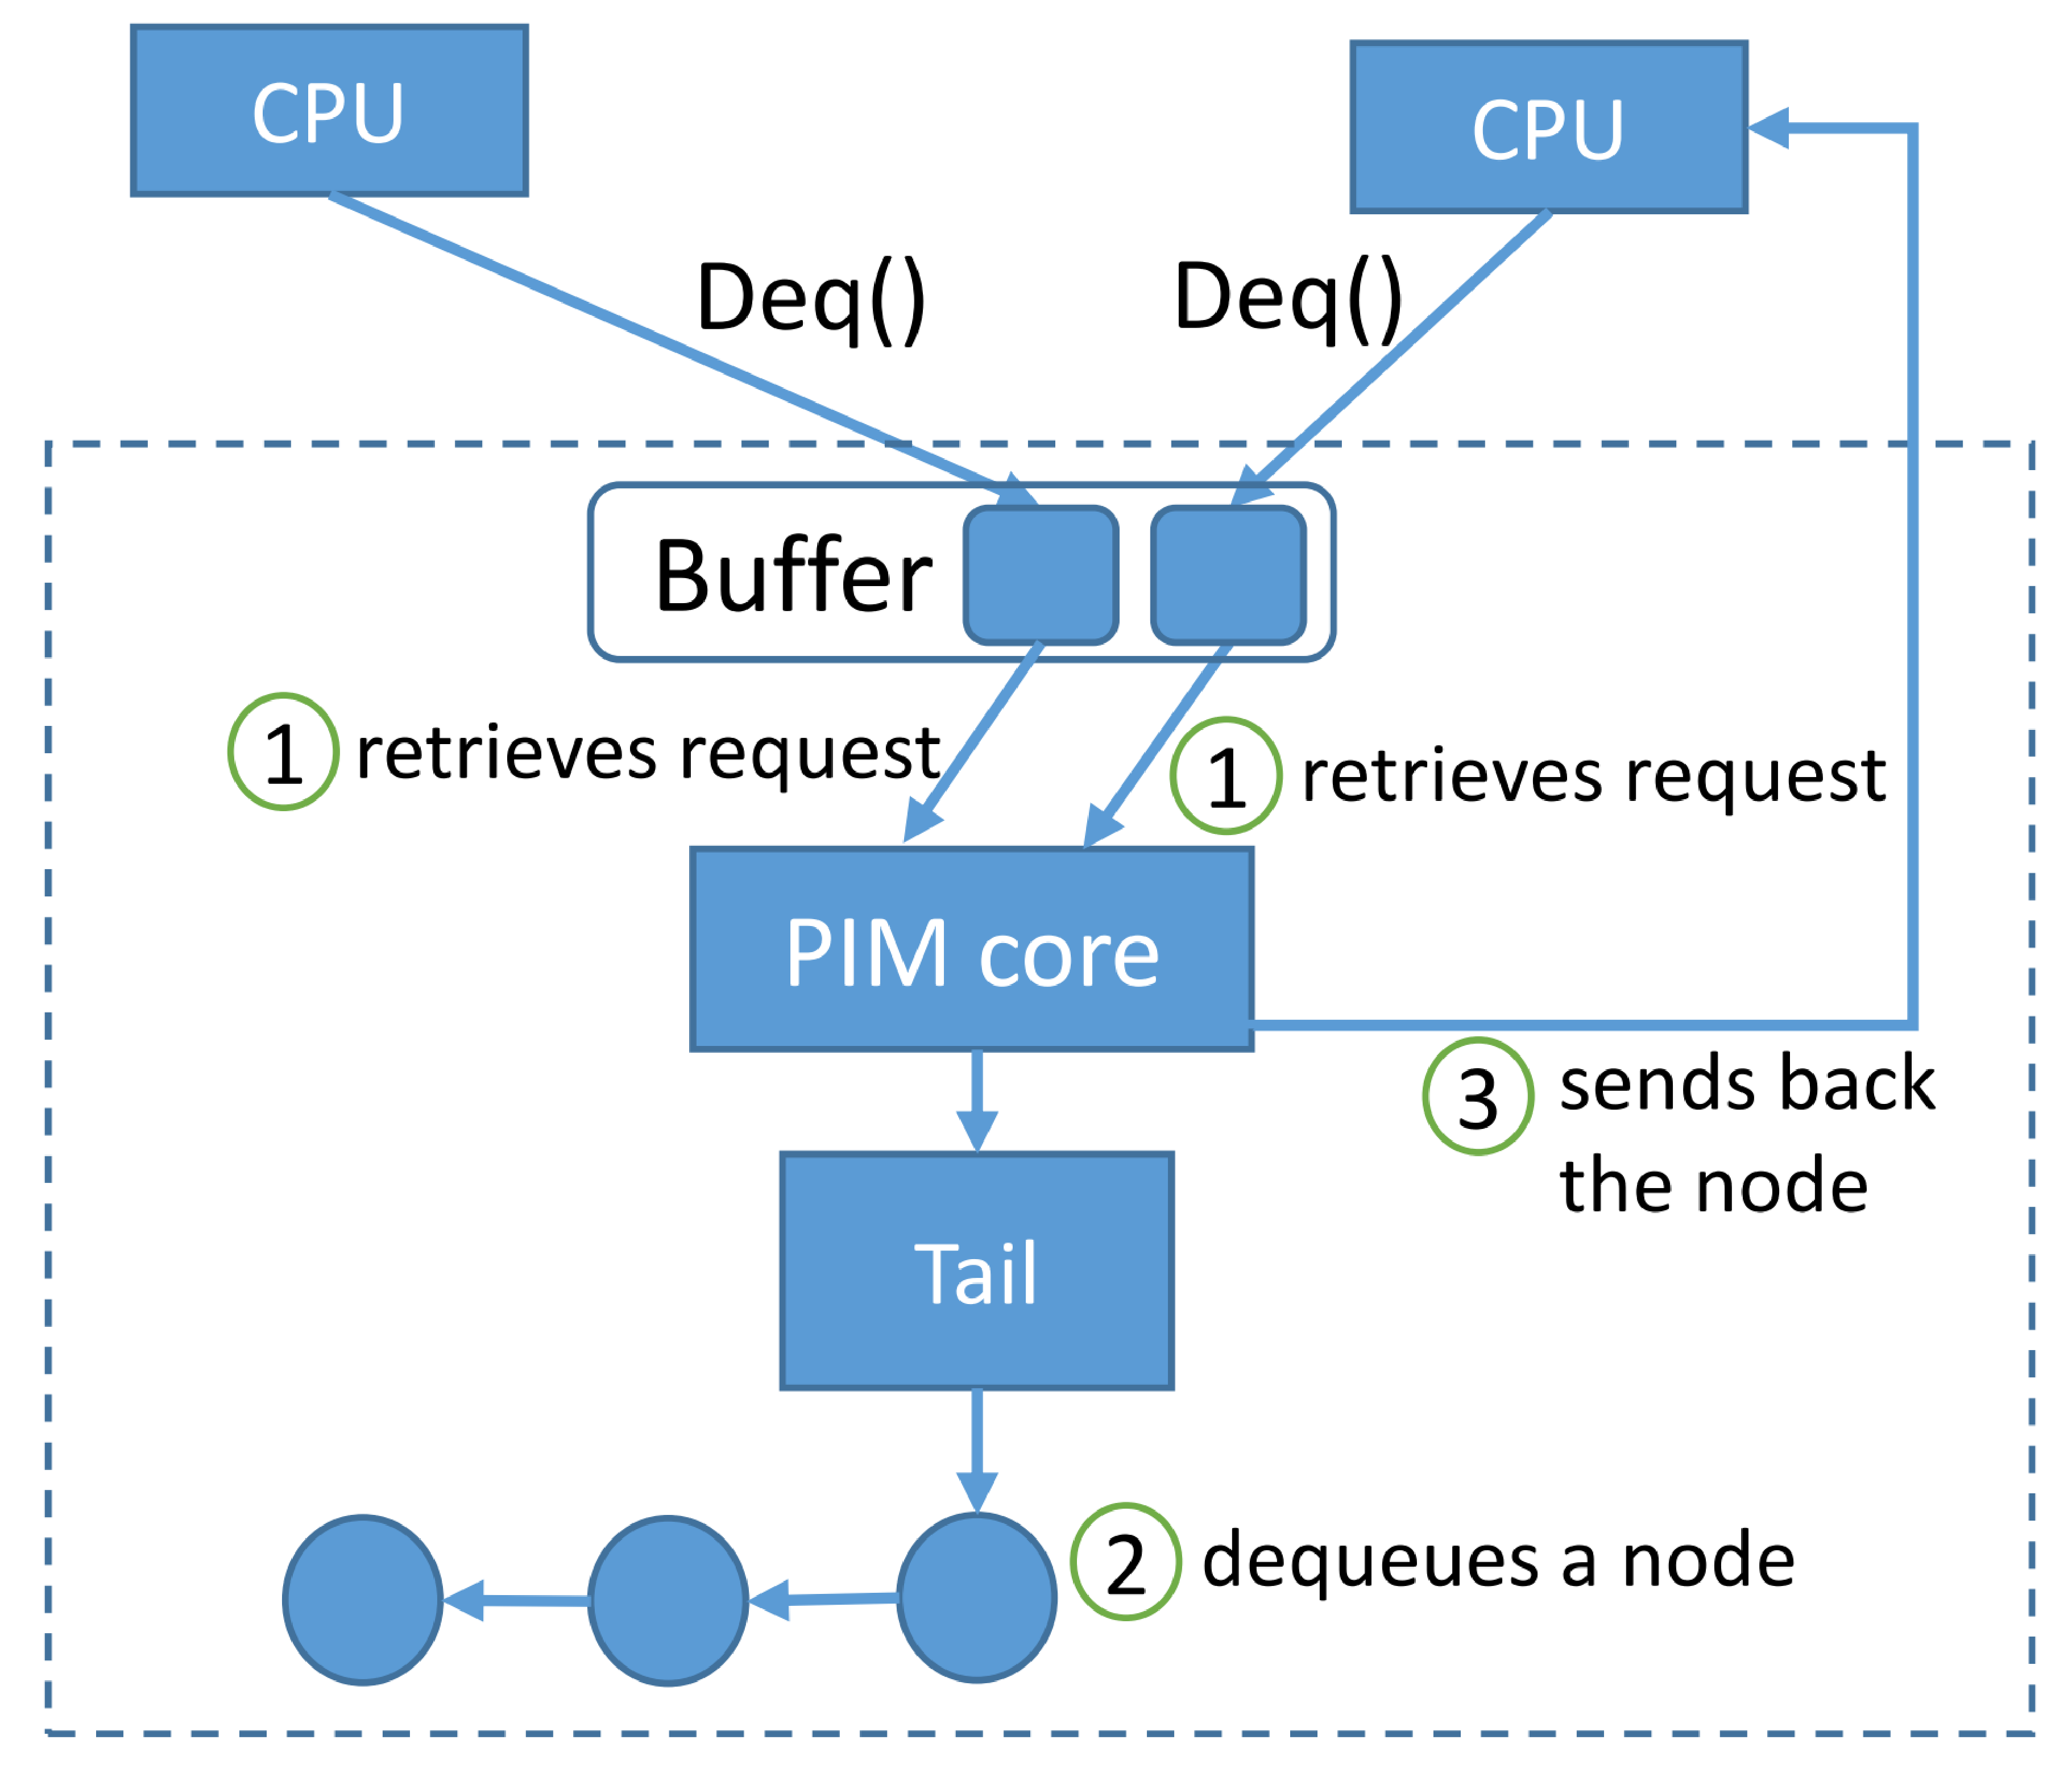
\includegraphics[width=.6\linewidth]{queue_pipeline.eps}}
\\
\subfigure[]{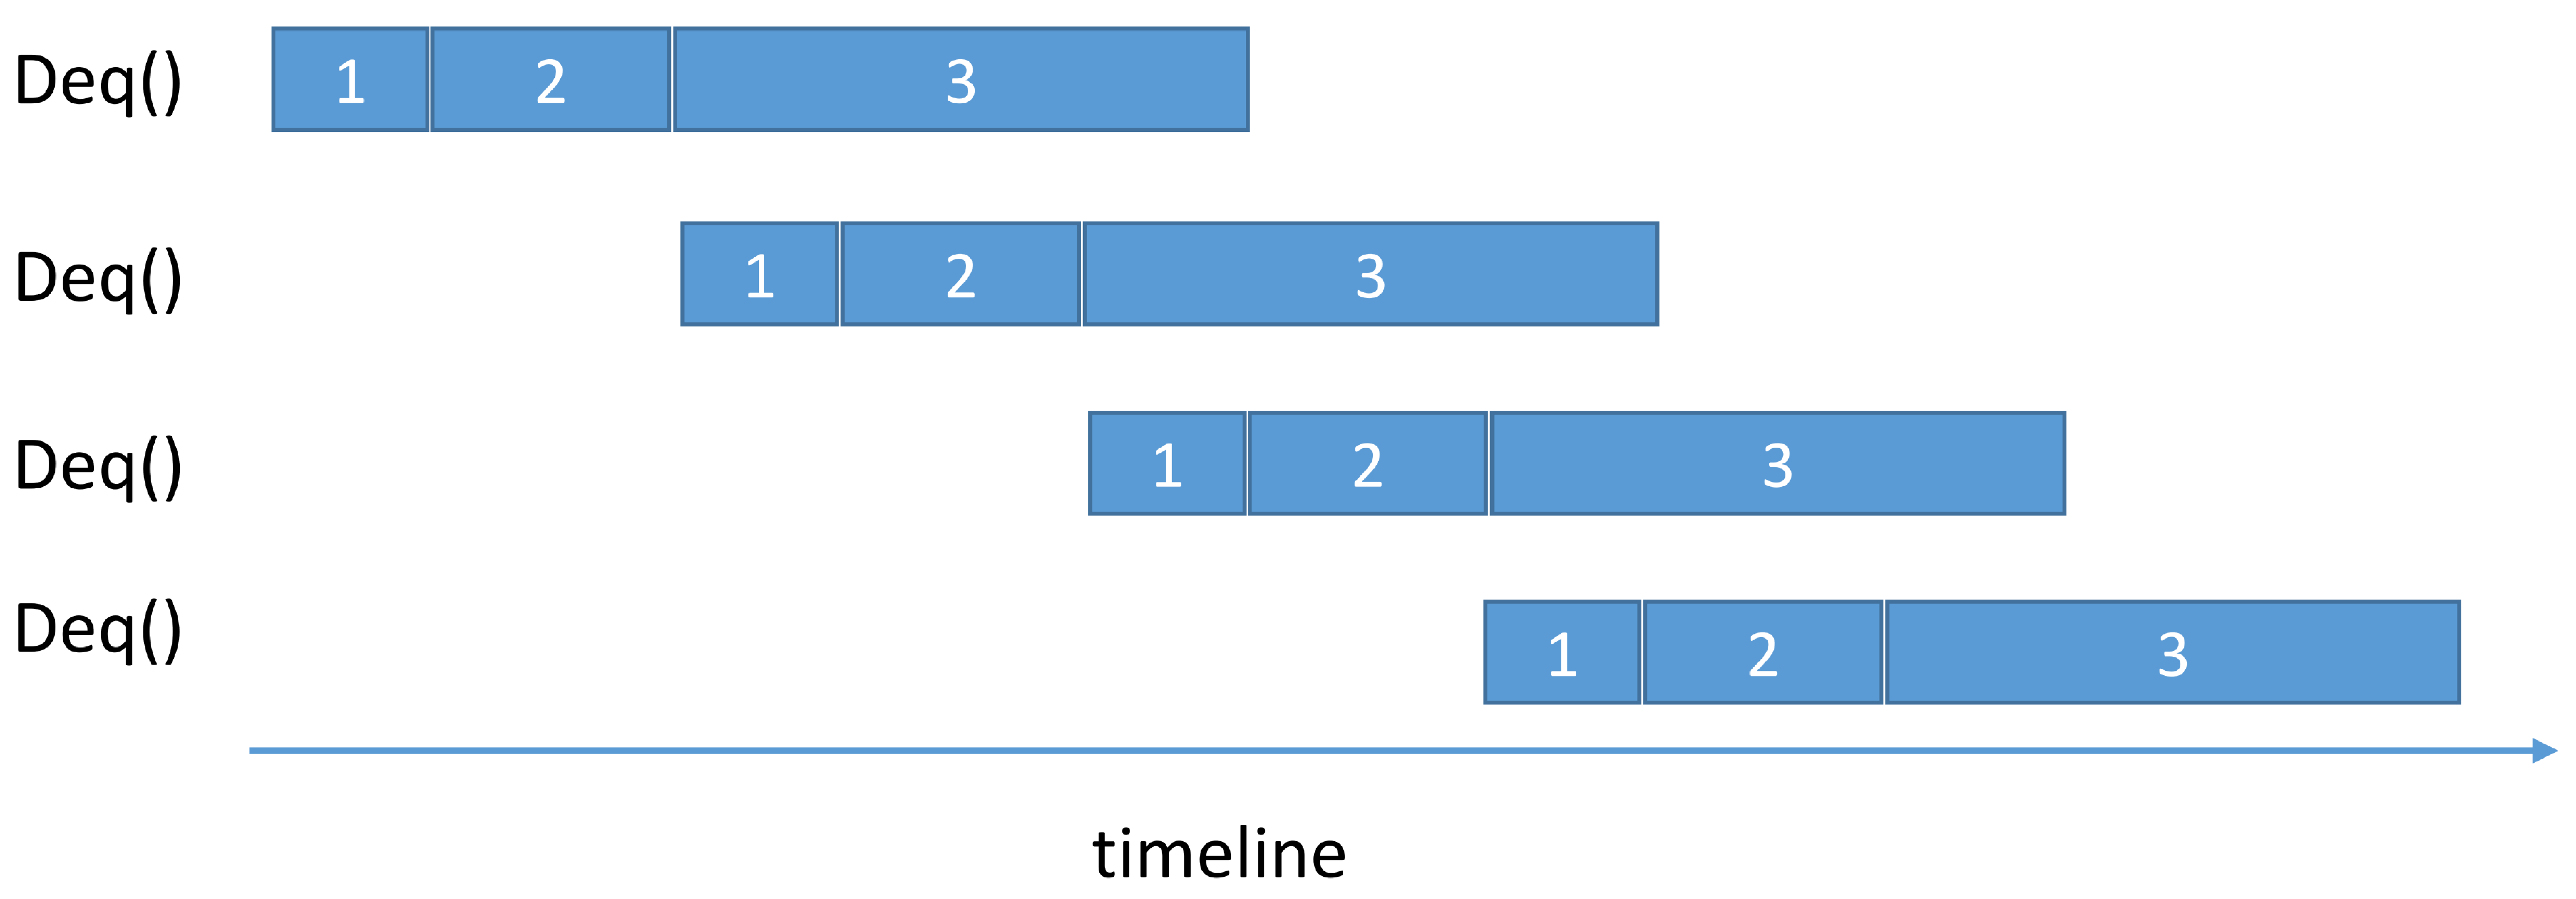
\includegraphics[width=.7\linewidth]{queue_pipeline_timeline.eps}}

%$\hrulefill$
\caption{(a) The pipelining optimization, where a PIM core can start executing 
a new deq() (step 1 of deq() for CPU B), without waiting for the dequeued node of 
the previous deq() to return to CPU A (step 3). 
(b) The timeline of pipelining four deq() requests.}
\label{figure:queue_pipeline}
\end{figure}
 
The throughput of a PIM core is given by the costs of its memory accesses and local computations, 
as long as it has enough bandwidth to keep sending messages back to CPUs.  
In this FIFO queue algorithm, the PIM core sends a single small message per request, 
so bandwidth is unlikely to become a bottleneck. 

Figure \ref{figure:queue_pipeline}(b) illustrates that 
the execution time of $p$ requests is the sum of the execution times of the first two steps 
for the $p$ requests, plus the message transfer time of step 3 for the last request.   
During steps 1-2 of a dequeue, the PIM core only makes one memory access to read the node 
to be dequeued, and two L1 cache accesses to read and modify the tail node of the dequeue segment.   
Therefore, the total execution time of $p$ requests, 
including the time $\latmes$ that the CPUs spend in sending their requests to a PIM core concurrently at the beginning this execution, 
is $\latmes + p(\latpim + \epsilon) + \latmes$, 
where $p(\latpim + \epsilon)$ is the sum of the execution times of the first two steps 
for the $p$ requests, and the second $\latmes$ is message transfer time of step 3 for the last request. 
$\epsilon$ is the total latency of the PIM core making two L1 cache accesses and sending one message.  
$\epsilon$ is negligible in our performance model. 

Assume that each CPU makes another request immediately after it receives the result of its previous request 
and that there are enough (at least $2\latmes / \latpim$) CPUs sending requests.
We can prove that the PIM core can always find another request in its buffer after it executes one. 
Let $x$ be the throughput of the PIM core in one second.
By the same analysis as above, we have $\latmes + x(\latpim + \epsilon) + \latmes = 1$,  
where 1 represents one second.
Therefore, the throughput (per second) of the PIM-managed FIFO queue is approximately 
$$x = {1 - 2\latmes \over \latpim + \epsilon} \approx {1 - 2\latmes \over \latpim} 
\approx {1 \over \latpim},$$
since $\latmes$ is usually only hundreds of nanoseconds and much smaller than 1 (second). 

Comparing the throughput values of the three FIFO queue algorithms, 
we can conclude that the PIM-managed FIFO queue with pipelining outperforms the other two FIFO queues 
when $2r_1 / r_2 > 1$ and $r_1 r_3 > 1$. 
If we assume $r_1 = r_2 = 3$ and $r_3 = 1$, then the throughput of our PIM-managed FIFO queue is expected to be 
twice the throughput of the flat-combining queue and three times that
of the F\&A queue.\footnote{ This does not imply that the F\&A queue is faster than the flat combining queue, 
since we only consider part of the costs of these queues in our analysis.}

When the PIM-managed FIFO queue is short, it may contain only one segment 
which deals with both enqueue and dequeue requests. 
In this case, its throughput is only half of the throughput shown above, 
but it is still at least as good as the throughput of the other two FIFO queues. 


\section{Related Work}
\label{section:related_work}
The PIM model is undergoing a renaissance. 
Studied for decades 
(e.g., \cite{Stone1970, Kogge1994, Gokhale1995, Patterson1997, Oskin1998, KangHYKGLTP99, Hall1999}), 
this model has recently re-emerged due to advances in 3D-stacked techology that 
can stack memory dies on top of a logic layer \cite{jeddeloh2012, Loh2008, Black2006}. 
For example, Micron and others have recently released a PIM prototype called 
the \emph{Hybrid Memory Cube} \cite{website:HMC}, and the model has again become the focus of architectural research.
Different PIM-based architectures have been proposed, either for general purposes or for 
specific applications \cite{Ahn2015:1, Ahn2015:2, Zhang2014:TTP, hsieh2016accelerating,
Azarkhish16, Akin2015:DRM, Azarkhish2015, AzarkhishPRLB17, boroumand2016, ZhuASSHPF13, ZhuGSPF13}.

The PIM model has many advantages, including low energy consumption and high bandwidth 
(e.g., \cite{Ahn2015:2, Zhang2014:TTP, ZhuASSHPF13, AzarkhishPRLB17}). 
Here, we focus on one more: low memory access latency 
\cite{Loh2008, hsieh2016accelerating, Azarkhish16}.
To our knowledge, however, we are the first to utilize PIM memory for designing efficient 
concurrent data structures. 
Although some researchers have studied how PIM memory can help speed up concurrent 
operations to data structures, such as parallel graph processing \cite{Ahn2015:2} and  
parallel pointer chasing on linked data structures \cite{hsieh2016accelerating}, 
the applications they consider require very simple, if any, synchronization between operations. 
In contract, operations to concurrent data structures can interleave in arbitrary orders, 
and therefore have to correctly synchronize with one another in all possible situations. 
This makes designing concurrent data structures with correctness guarantees like 
linearizability \cite{Herlihy90} very challenging. 

Moreover, no one has ever compared the performance of data structures in the PIM model 
with that of state-of-the-art concurrent data structures in the classic shared memory model. 
We analyze and evaluate concurrent linked-lists and skip-lists, 
as representatives of pointer-chasing data structures, and concurrent FIFO queues, 
as representatives of contended data structures.
For linked-lists, we compare our PIM-managed implementation with well-known approaches 
such as fine-grained locking \cite{Heller05} and flat combining \cite{Hendler10}.

For skip-lists, we compare our implementation with the lock-free skip-list \cite{Herlihy08} 
and a skip-list with flat combining and partitioning optimization. 
For FIFO queues, we compare our implementation with the flat-combining FIFO queue 
\cite{Hendler10} and the F\&A-based FIFO queue \cite{Morrison13}. 
\section{Conclusion}
\label{section:conclusion}

In this paper, we study how to design efficient data structures that
can take advantage of the promising benefits offered by the Processing
in Memory (PIM) paradigm.  We analyze and compare the performance of
our new PIM-managed data structures with traditional concurrent data
structures that were proposed in the literature to take advantage of
multiple processors.  To this end, we develop a simplified performance
model for PIM.  Using this model, along with empirical performance
measurements from a modern system, we show that naive PIM-managed data
structures \emph{cannot} outperform traditional concurrent data
structures, due to the lack of parallelism and the high communication
cost between the CPUs and the PIM cores.  To improve the performance
of PIM data structures, we propose novel designs for low-contention
pointer-chasing data structures, such as linked-lists and skip-lists,
and for contended data structures, such as FIFO queues.  We show that
our new PIM-managed data structures can outperform state-of-the-art
concurrent data structures, making PIM memory a promising platform for
managing data structures. We conclude that it is very promising to
examine novel data structure designs for the PIM paradigm, and hope
future work builds upon our analyses to develop other types of
PIM-managed data structures.

 


%\bibliographystyle{ACM-Reference-Format}
\bibliographystyle{plain}
\bibliography{refs_pim}

\end{document}

